
\begin{table}[ht]
	\centering
	\renewcommand{\arraystretch}{1.5}
	\setlength{\tabcolsep}{15pt}
	\resizebox{\textwidth}{!}{
	\begin{tabular}{lllll}
		\hline
		\rowcolor[HTML]{EFEFEF} 
		\multicolumn{1}{c}{\cellcolor[HTML]{EFEFEF}\textbf{Flag}} & \multicolumn{4}{c}{\cellcolor[HTML]{EFEFEF}\textbf{Descrição}}                                               \\ \hline
		RF1                                                       & \multicolumn{4}{l}{Verificação dos preços contratuais para ajustes diretos.}                                 \\
		RF2                                                       & \multicolumn{4}{l}{Comparação entre o preço base e o preço total efetivo.}             \\
		RF3                                                       & \multicolumn{4}{l}{Análise da publicação de anúncios em datas não convencionais.}                            \\
		R003                                                      & \multicolumn{4}{l}{Análise do prazo de apresentação de propostas.}                                           \\
		R017                                                      & \multicolumn{4}{l}{Análise do preço contratual, por grupo de CPV.}                    \\
		R018                                                      & \multicolumn{4}{l}{Análise de concursos públicos com uma entidade concorrente.}                              \\
		R019                                                      & \multicolumn{4}{l}{Análise do número de entidades concorrentes.}                       \\ \hline
		{\textit{R031}}                                       & \multicolumn{4}{l}{{ \textit{Comparação entre o preço base e o preço contratual.}}} \\
		{\textit{R051}}                                       & \multicolumn{4}{l}{{ \textit{Análise da concentração de mercado.}}}                                       \\ \hline
	\end{tabular}%
	}
	\caption{Conjunto de flags desenvolvidas.}
	\label{tab:flags}
\end{table}


O processo de automação aplicou as flags desenvolvidas a todos os contratos adicionadas à base de dados até ao início de julho. Porém, por motivos de consistência, só se analisaram os contratos celebrados até dia 1 de maio do presente ano civil, tal como foi estabelecido no Capítulo \ref{ch:variables}. 

A partir da Tabela \ref{final1}, podem-se observar o número de contratos inconformes detetados e a respetiva percentagem, para cada uma das \textit{flags} aplicadas ao longo deste processo. Do conjunto de \textit{flags} apresentadas, destacam-se a R017, R018 e R019, com uma percentagem de contratos inconformes identificados de 21\%, 19.9\% e 23.5\%, respetivamente. 

Nas Figuras \ref{final2}, \ref{final3}, \ref{final4}, \ref{final5} e \ref{final6} pode-se assitir à variação do número de contratos e respetiva percentagem, por ano, para cada \textit{flag}. À exceção das \textit{flag} RF3 e R018, todas elas detetam um maior número de inconformidades detetadas no ano de 2023. Presumivelmente, esta observação deve-se ao facto de ter sido neste ano civil onde se registou um maior número de contratos celebrados, tal como se contemplou na Figura \ref{fig:precocps1}.


\begin{table}[ht]
	\centering
	\renewcommand{\arraystretch}{1.5}
	\setlength{\tabcolsep}{15pt}
	\resizebox{\textwidth}{!}{
		\begin{tabular}{lclcccccc}
			\toprule[2px]
			\textbf{Tipo de Procedimento}                                                       & \multicolumn{2}{c}{Ajuste Direto} & \multicolumn{6}{c}{Concurso Público}       \\ \hline
			\textbf{Total de concursos}                                                         & \multicolumn{2}{c}{546903}        & \multicolumn{6}{c}{130099}                 \\ \midrule[1.5px]
			\textbf{Flag}                                                                       & \multicolumn{2}{c}{RF1}           & RF2 & RF3   & R003 & R017  & R018  & R019  \\ \hline
			\textbf{\begin{tabular}[c]{@{}l@{}}Número de \\ contratos inconformes\end{tabular}} & \multicolumn{2}{c}{16910}         & 0   & 11958 & 4751 & 27261 & 25853 & 30576 \\ \hline
			\textbf{Percentagem \%}                                                             & \multicolumn{2}{c}{3.1}           & 0   & 9.2   & 3.7  & 21    & 19.9  & 23.5  \\ \bottomrule[1.5px]
		\end{tabular}%
	}
	\caption{Número de contratos inconformes detetados para cada indicador construído.}
	\label{final1}
\end{table}



\begin{figure}[H]
	\centering
	\begin{minipage}{.48\linewidth}
		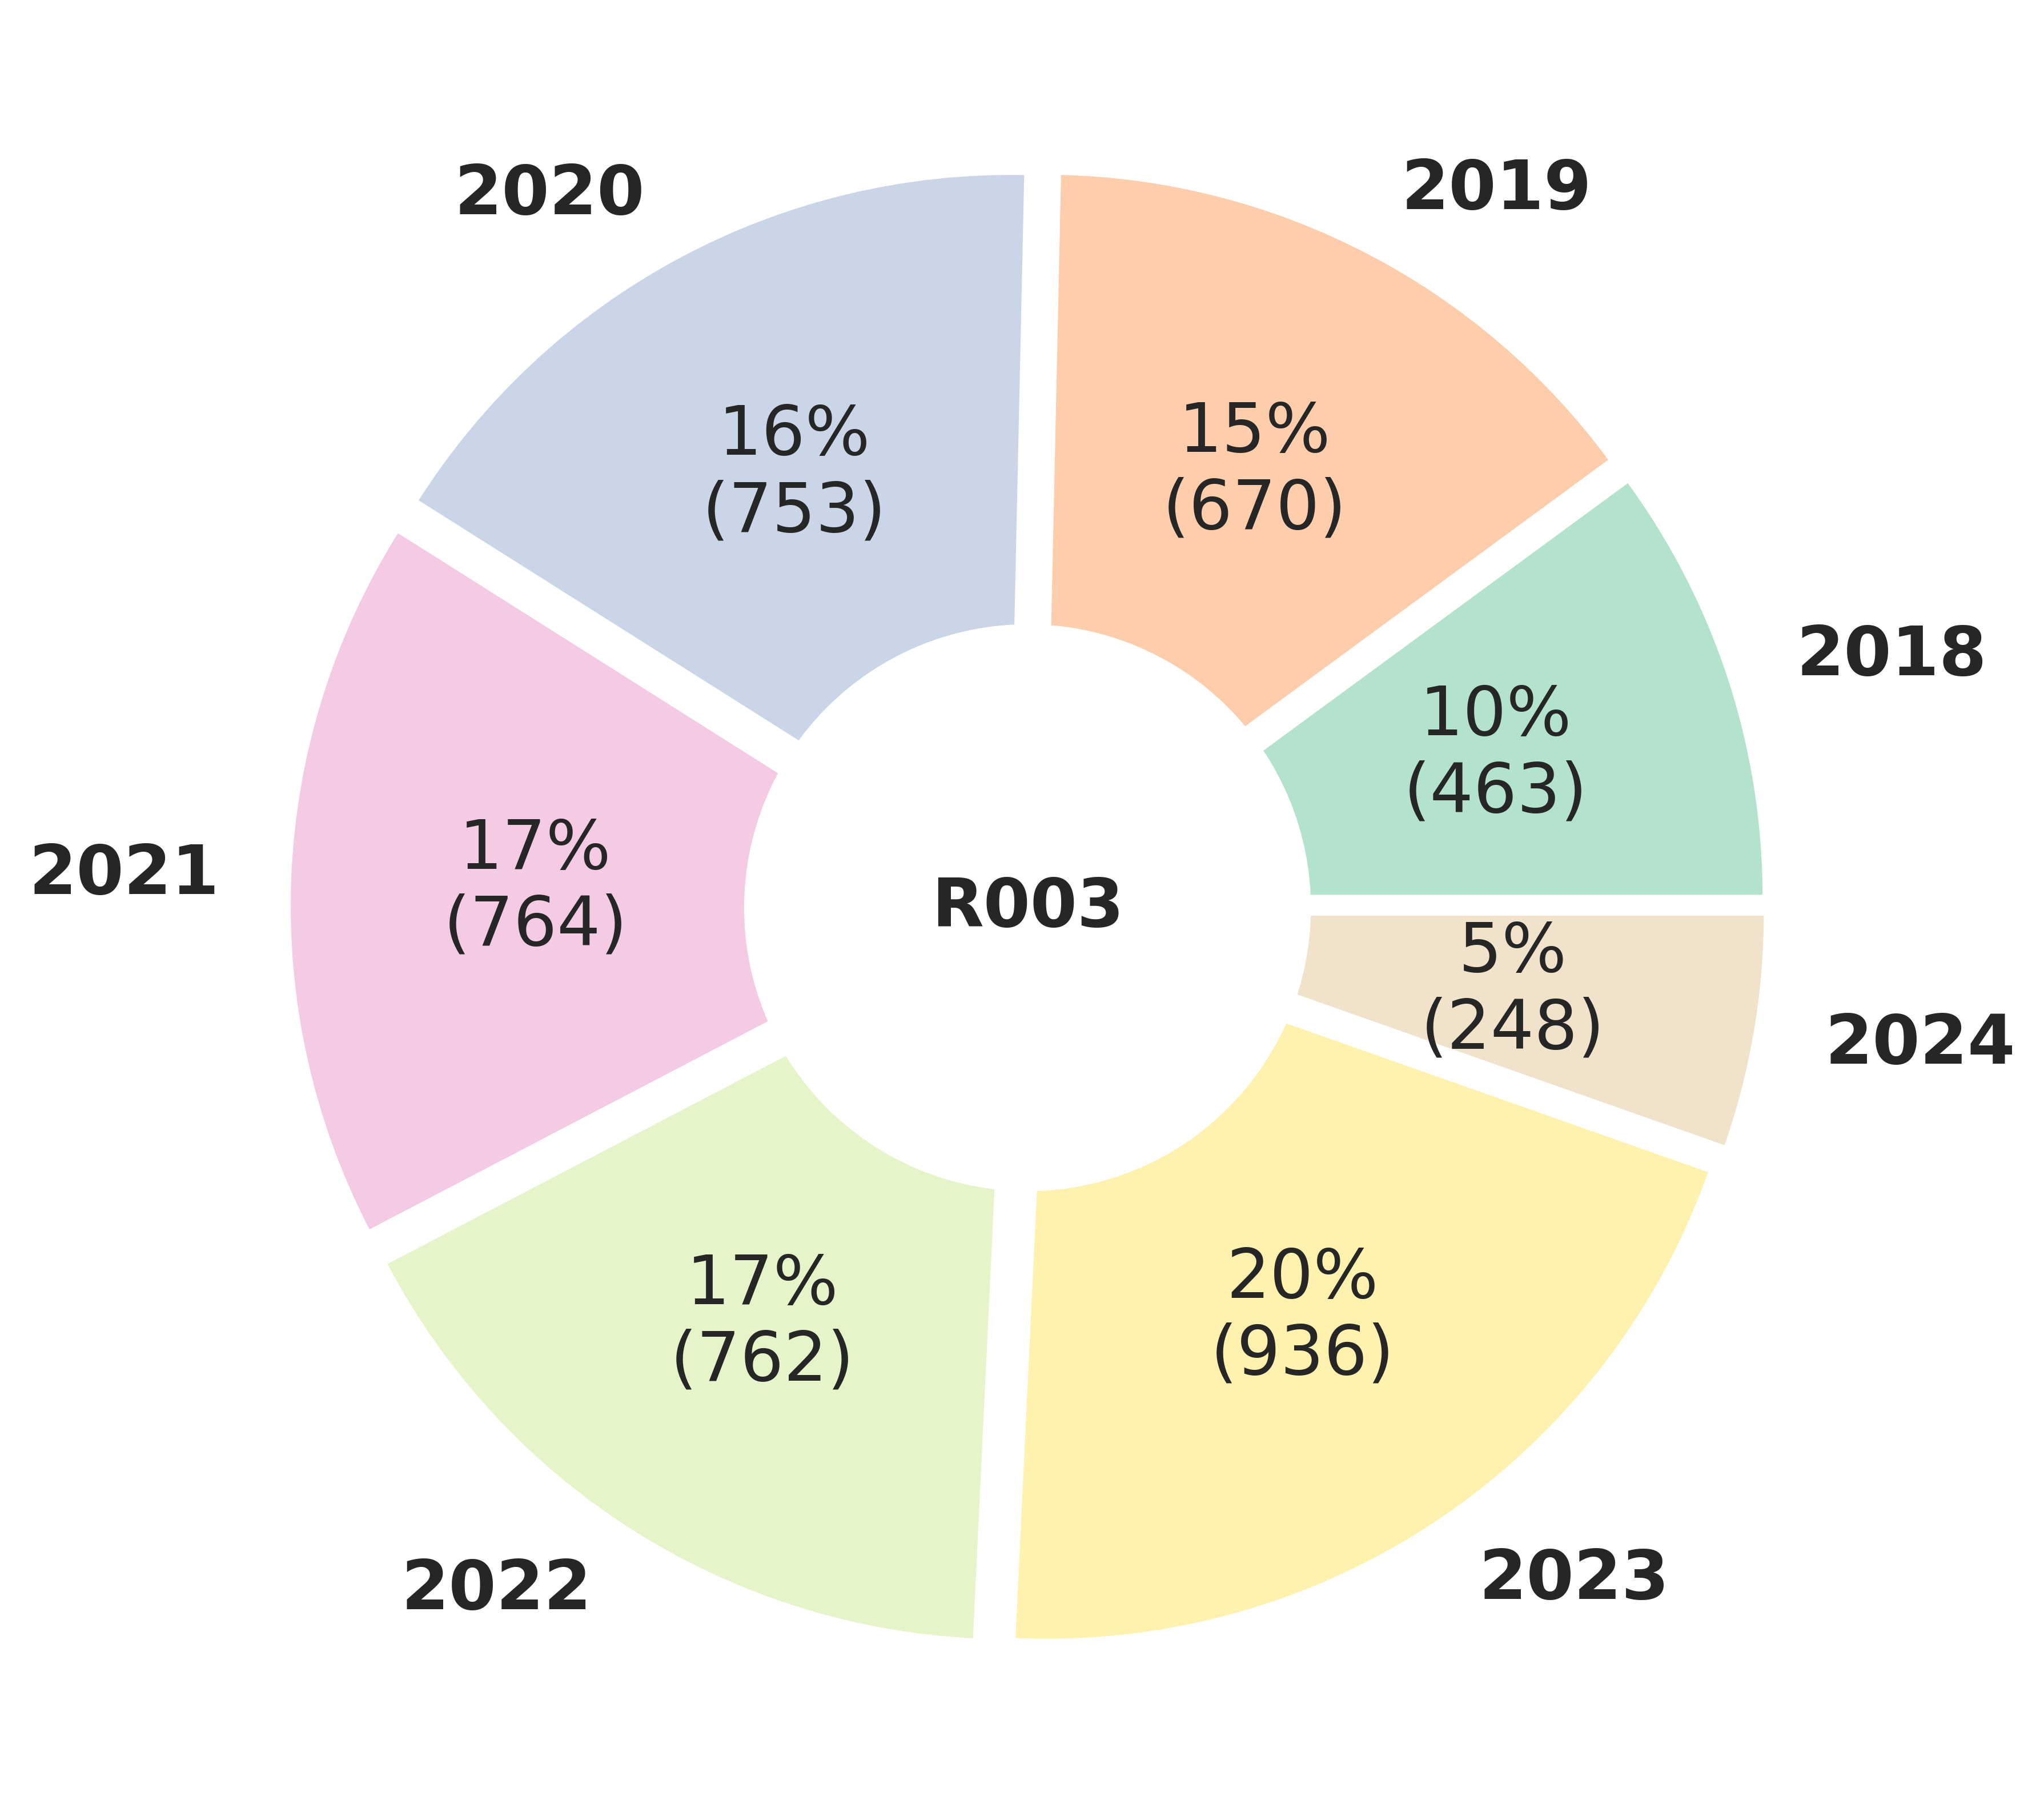
\includegraphics[width=\linewidth]{imagens/final/circle_R003.png}
		\caption{Número de contratos inconformes detetados para o indicador R003, por ano.}
		\label{final2}
	\end{minipage}
	\hfill
	\begin{minipage}{.48\linewidth}
		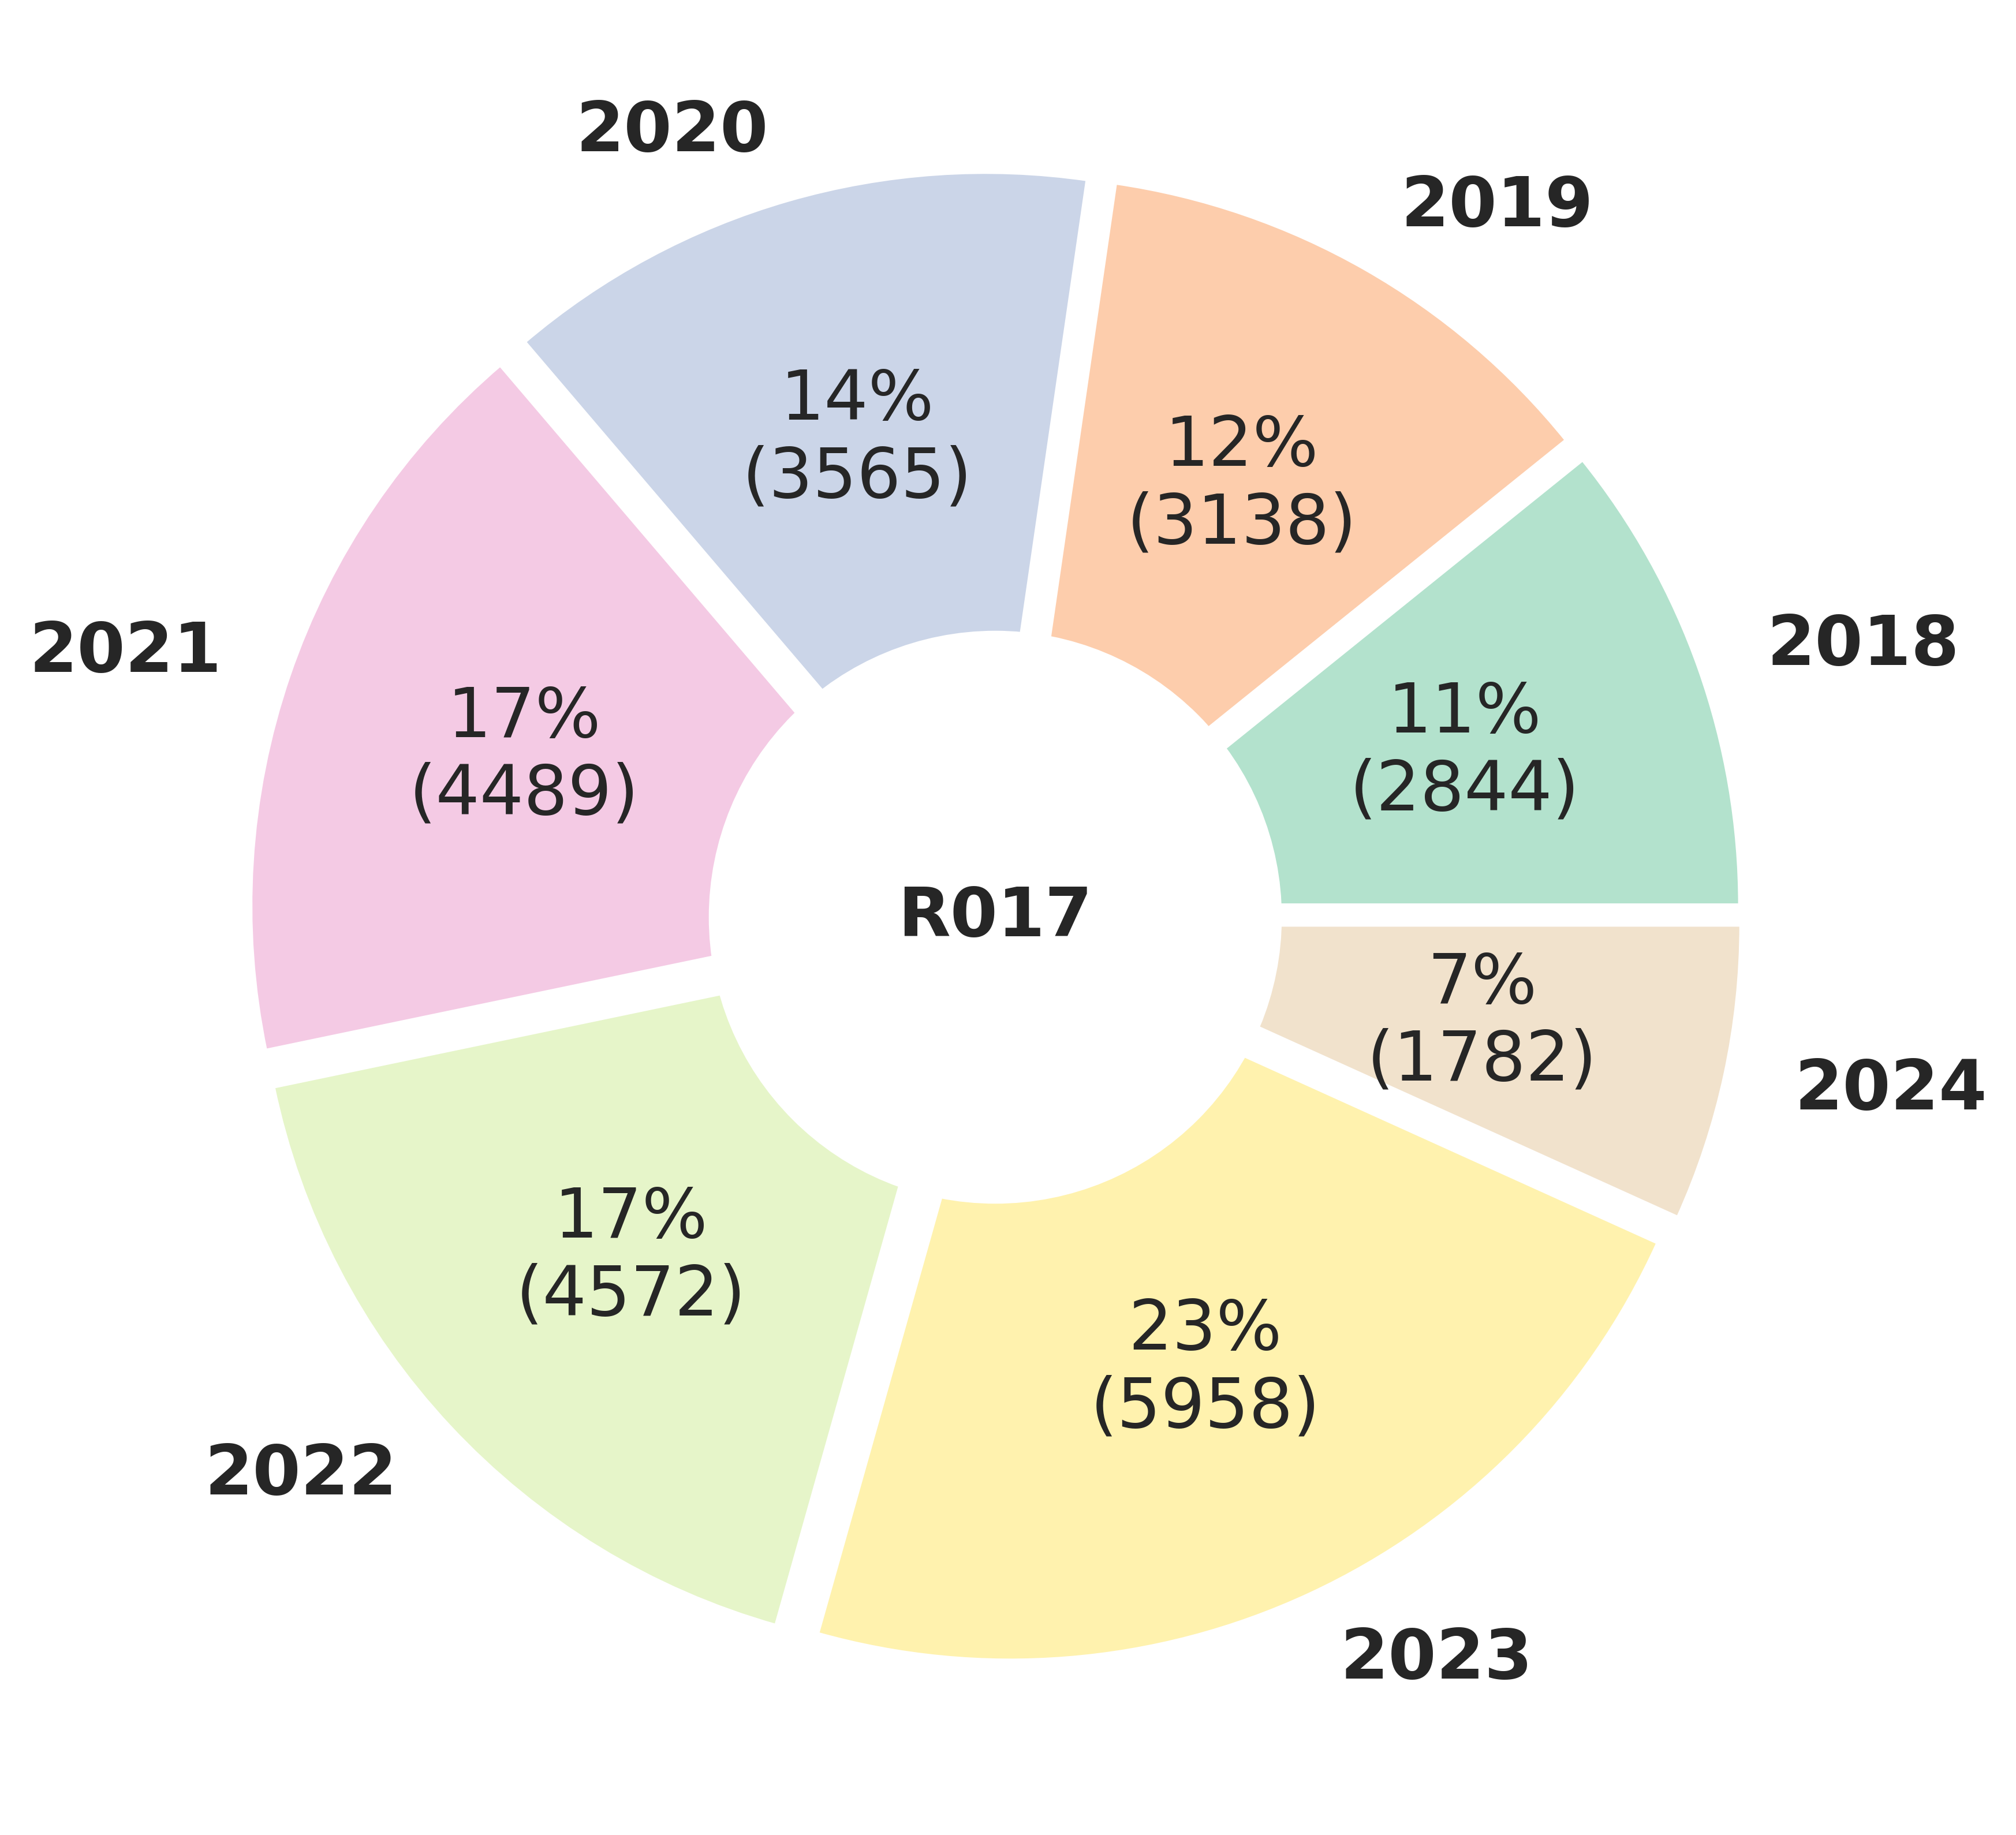
\includegraphics[width=\linewidth]{imagens/final/circle_R017.png}
		\caption{Número de contratos inconformes detetados para o indicador R017, por ano.}
		\label{final3}
		
	\end{minipage}
\end{figure}




\begin{figure}[H]
	\centering
	\begin{minipage}{.48\linewidth}
		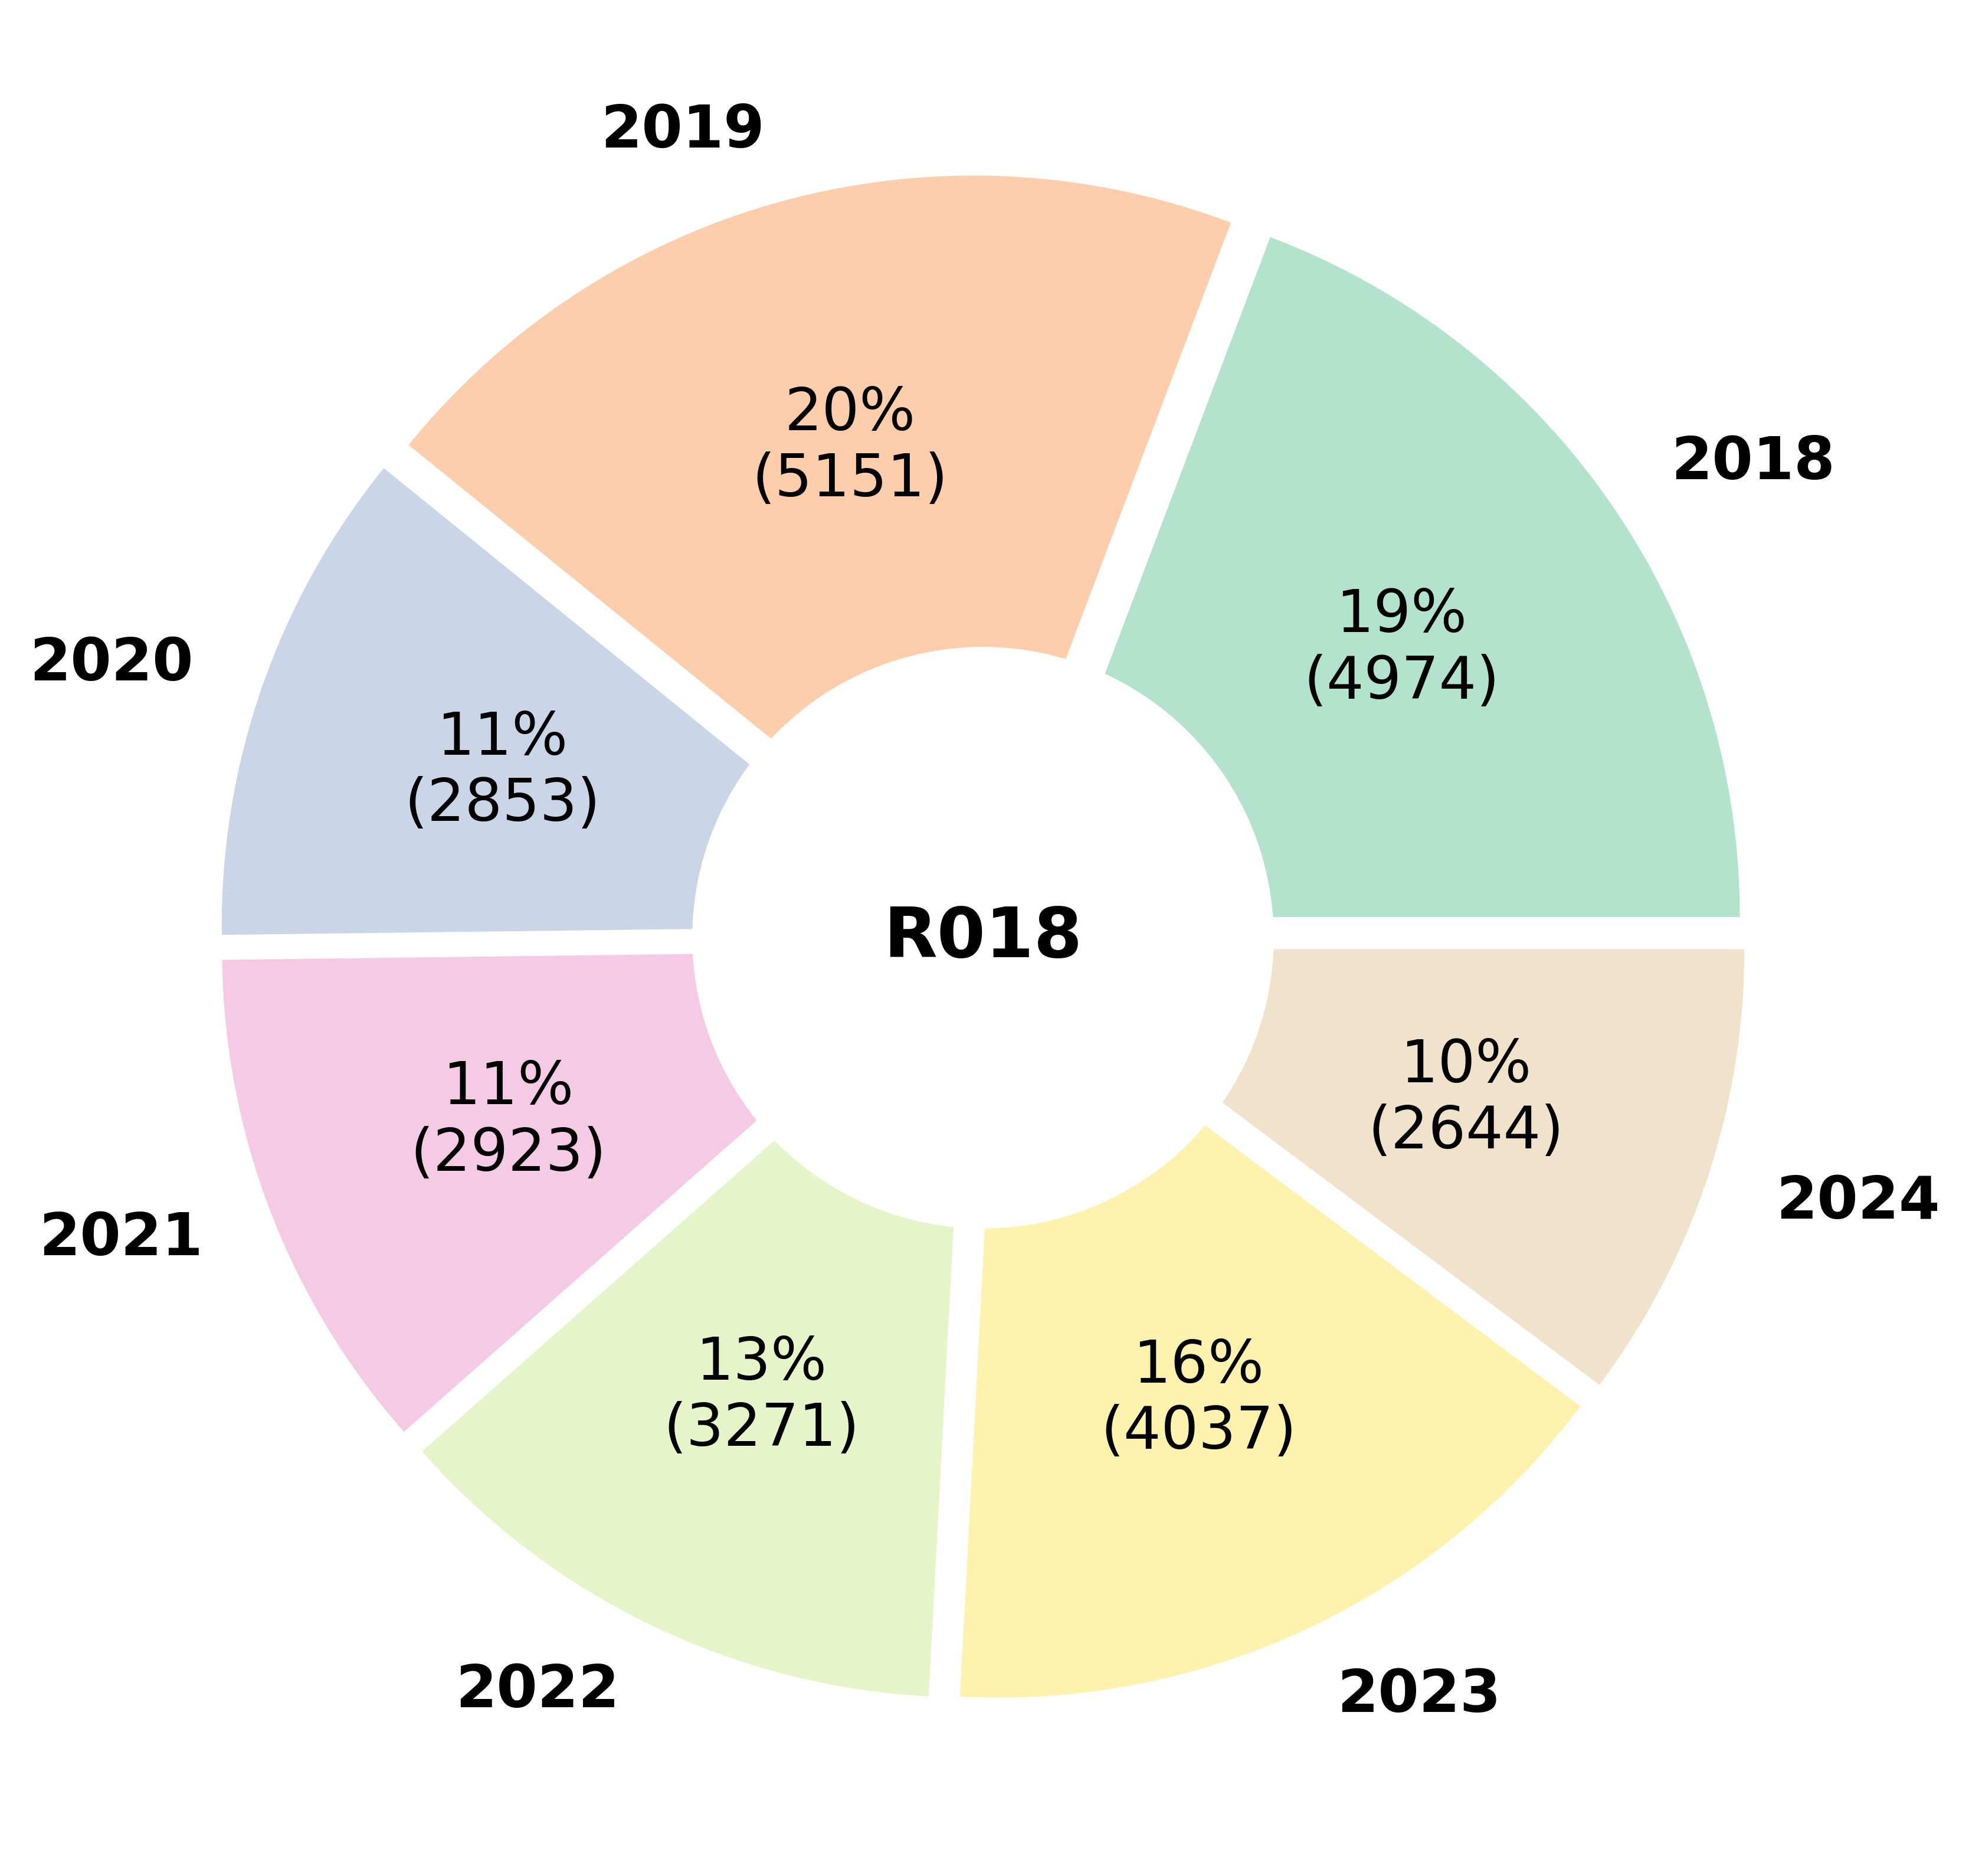
\includegraphics[width=\linewidth]{imagens/final/circle_R018.png}
		\caption{Número de contratos inconformes detetados para o indicador R018, por ano.}
		\label{final4}
		
	\end{minipage}
	\hfill
	\begin{minipage}{.48\linewidth}
		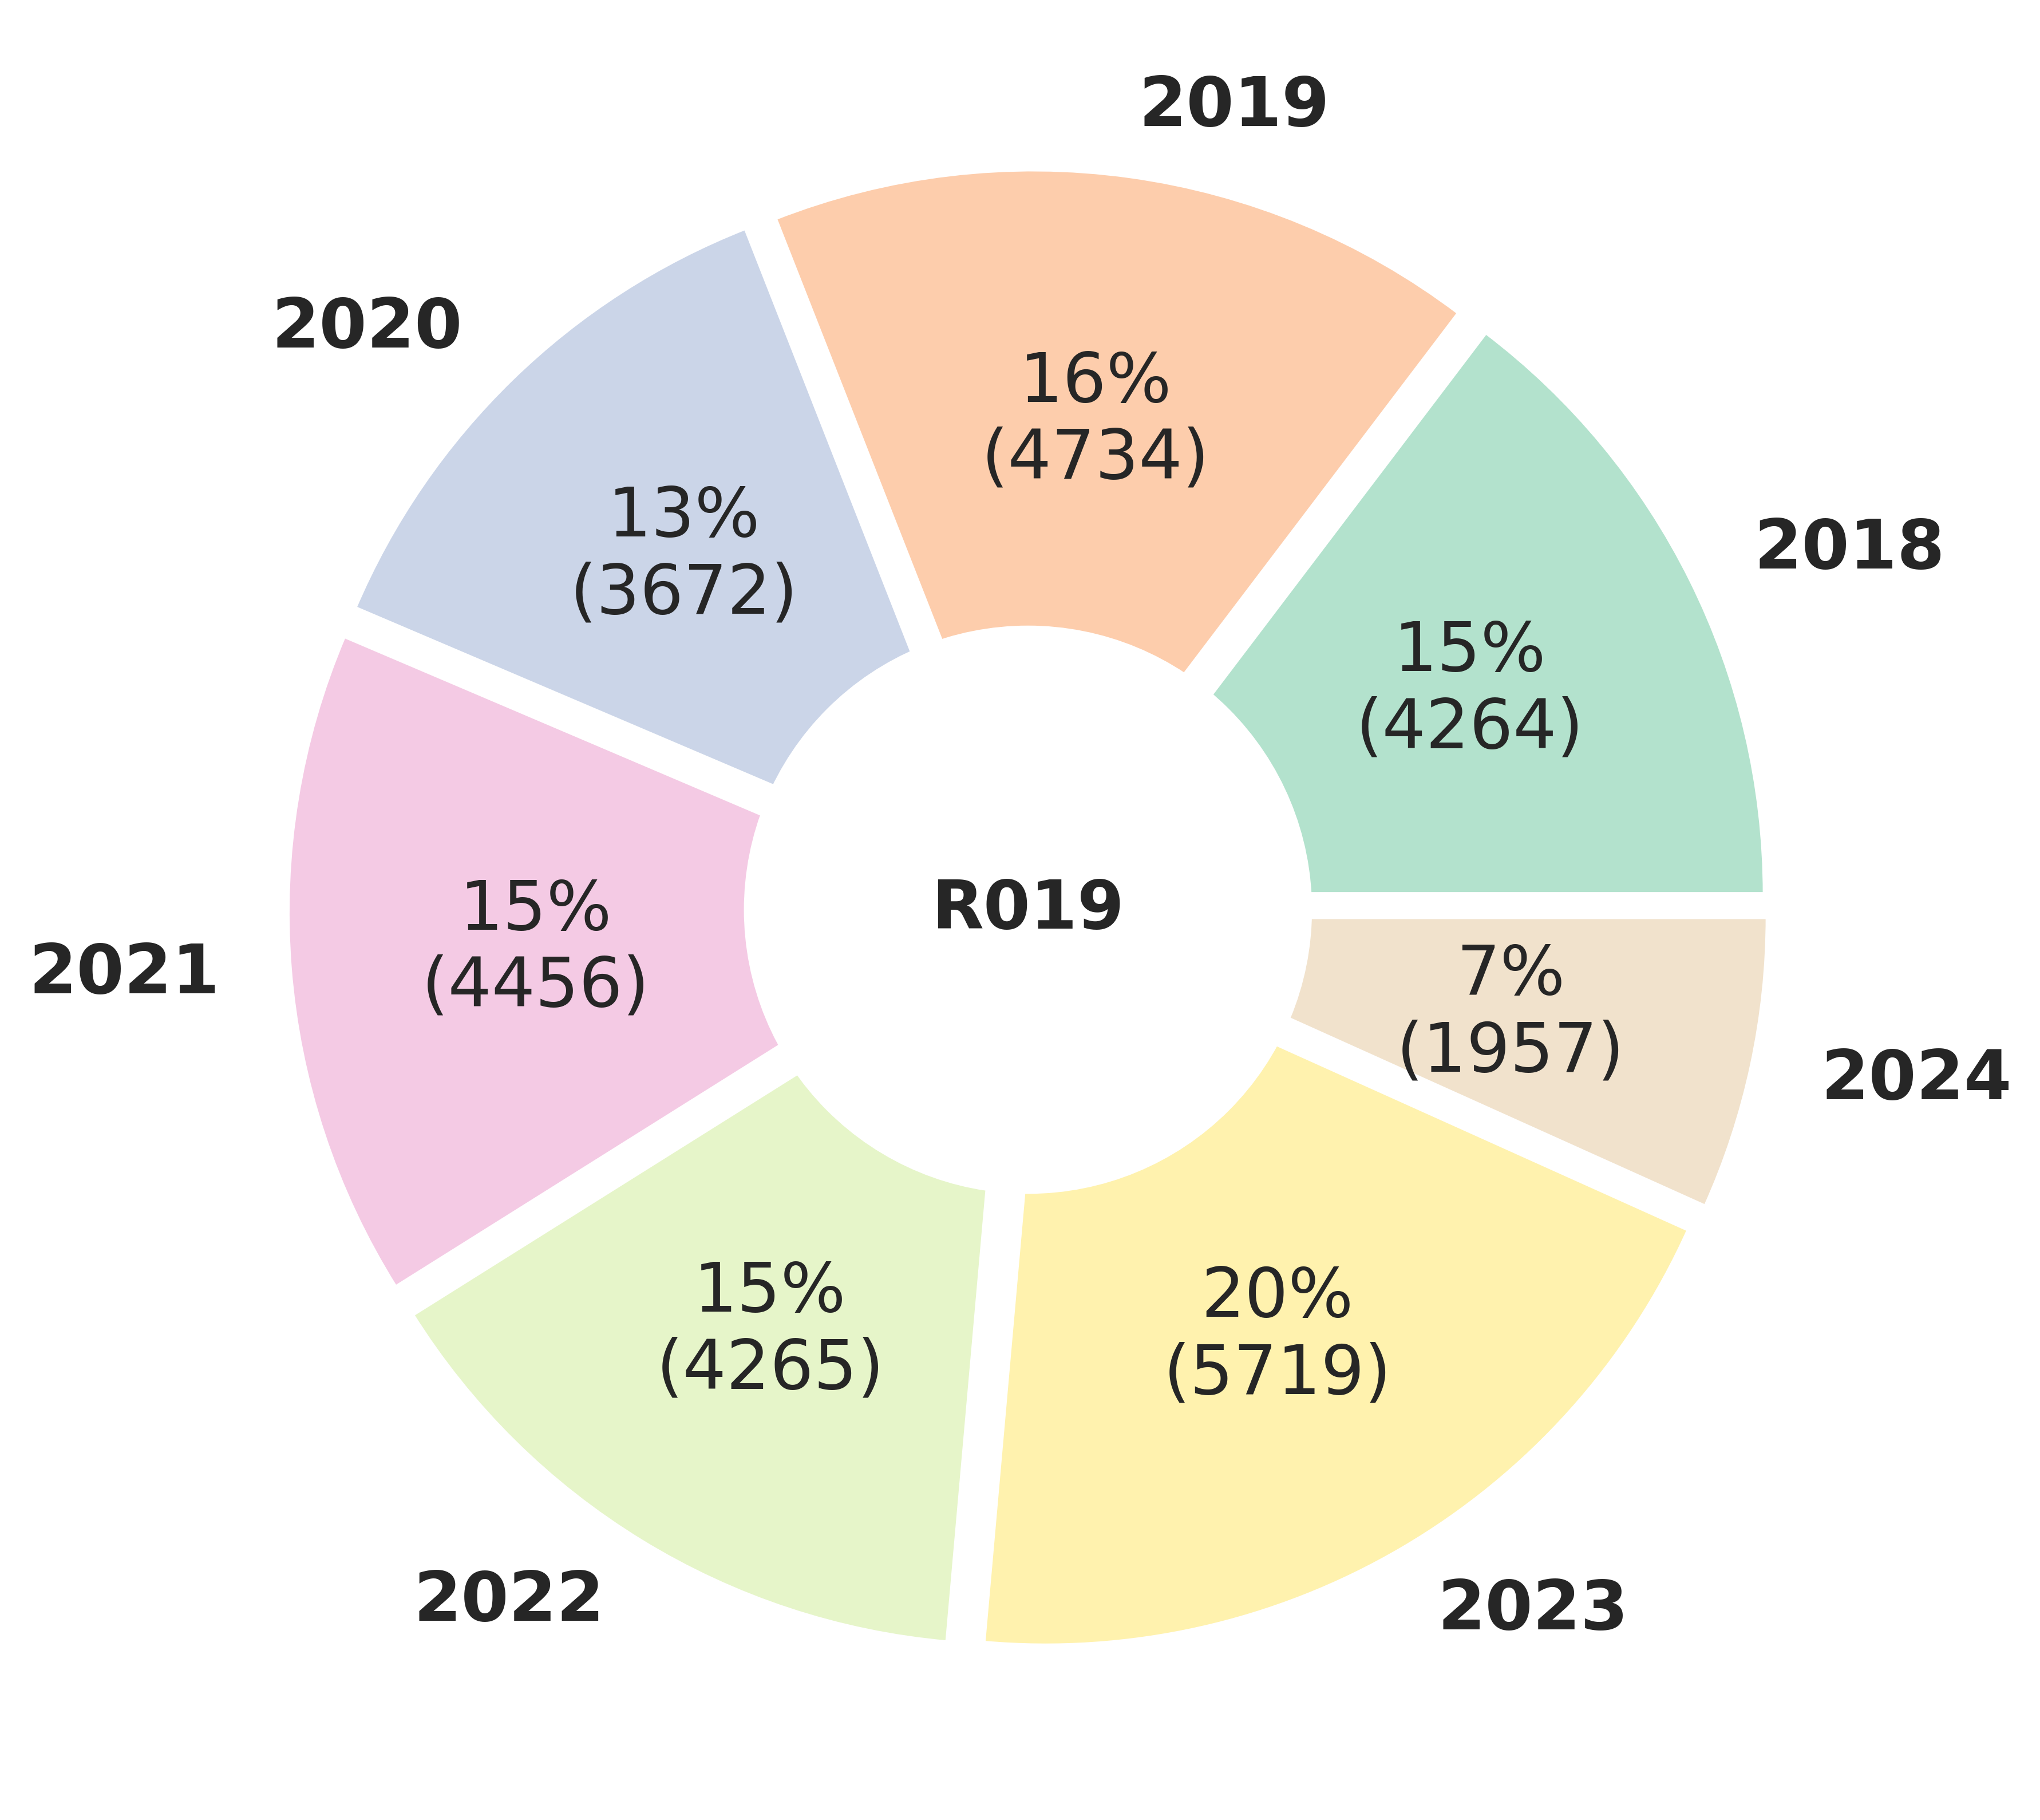
\includegraphics[width=\linewidth]{imagens/final/circle_R019.png}
		\caption{Número de contratos inconformes detetados para o indicador R019, por ano.}
		\label{final5}
				
	\end{minipage}
\end{figure}




\begin{figure}[H]
	\centering
	\begin{minipage}{.48\linewidth}
		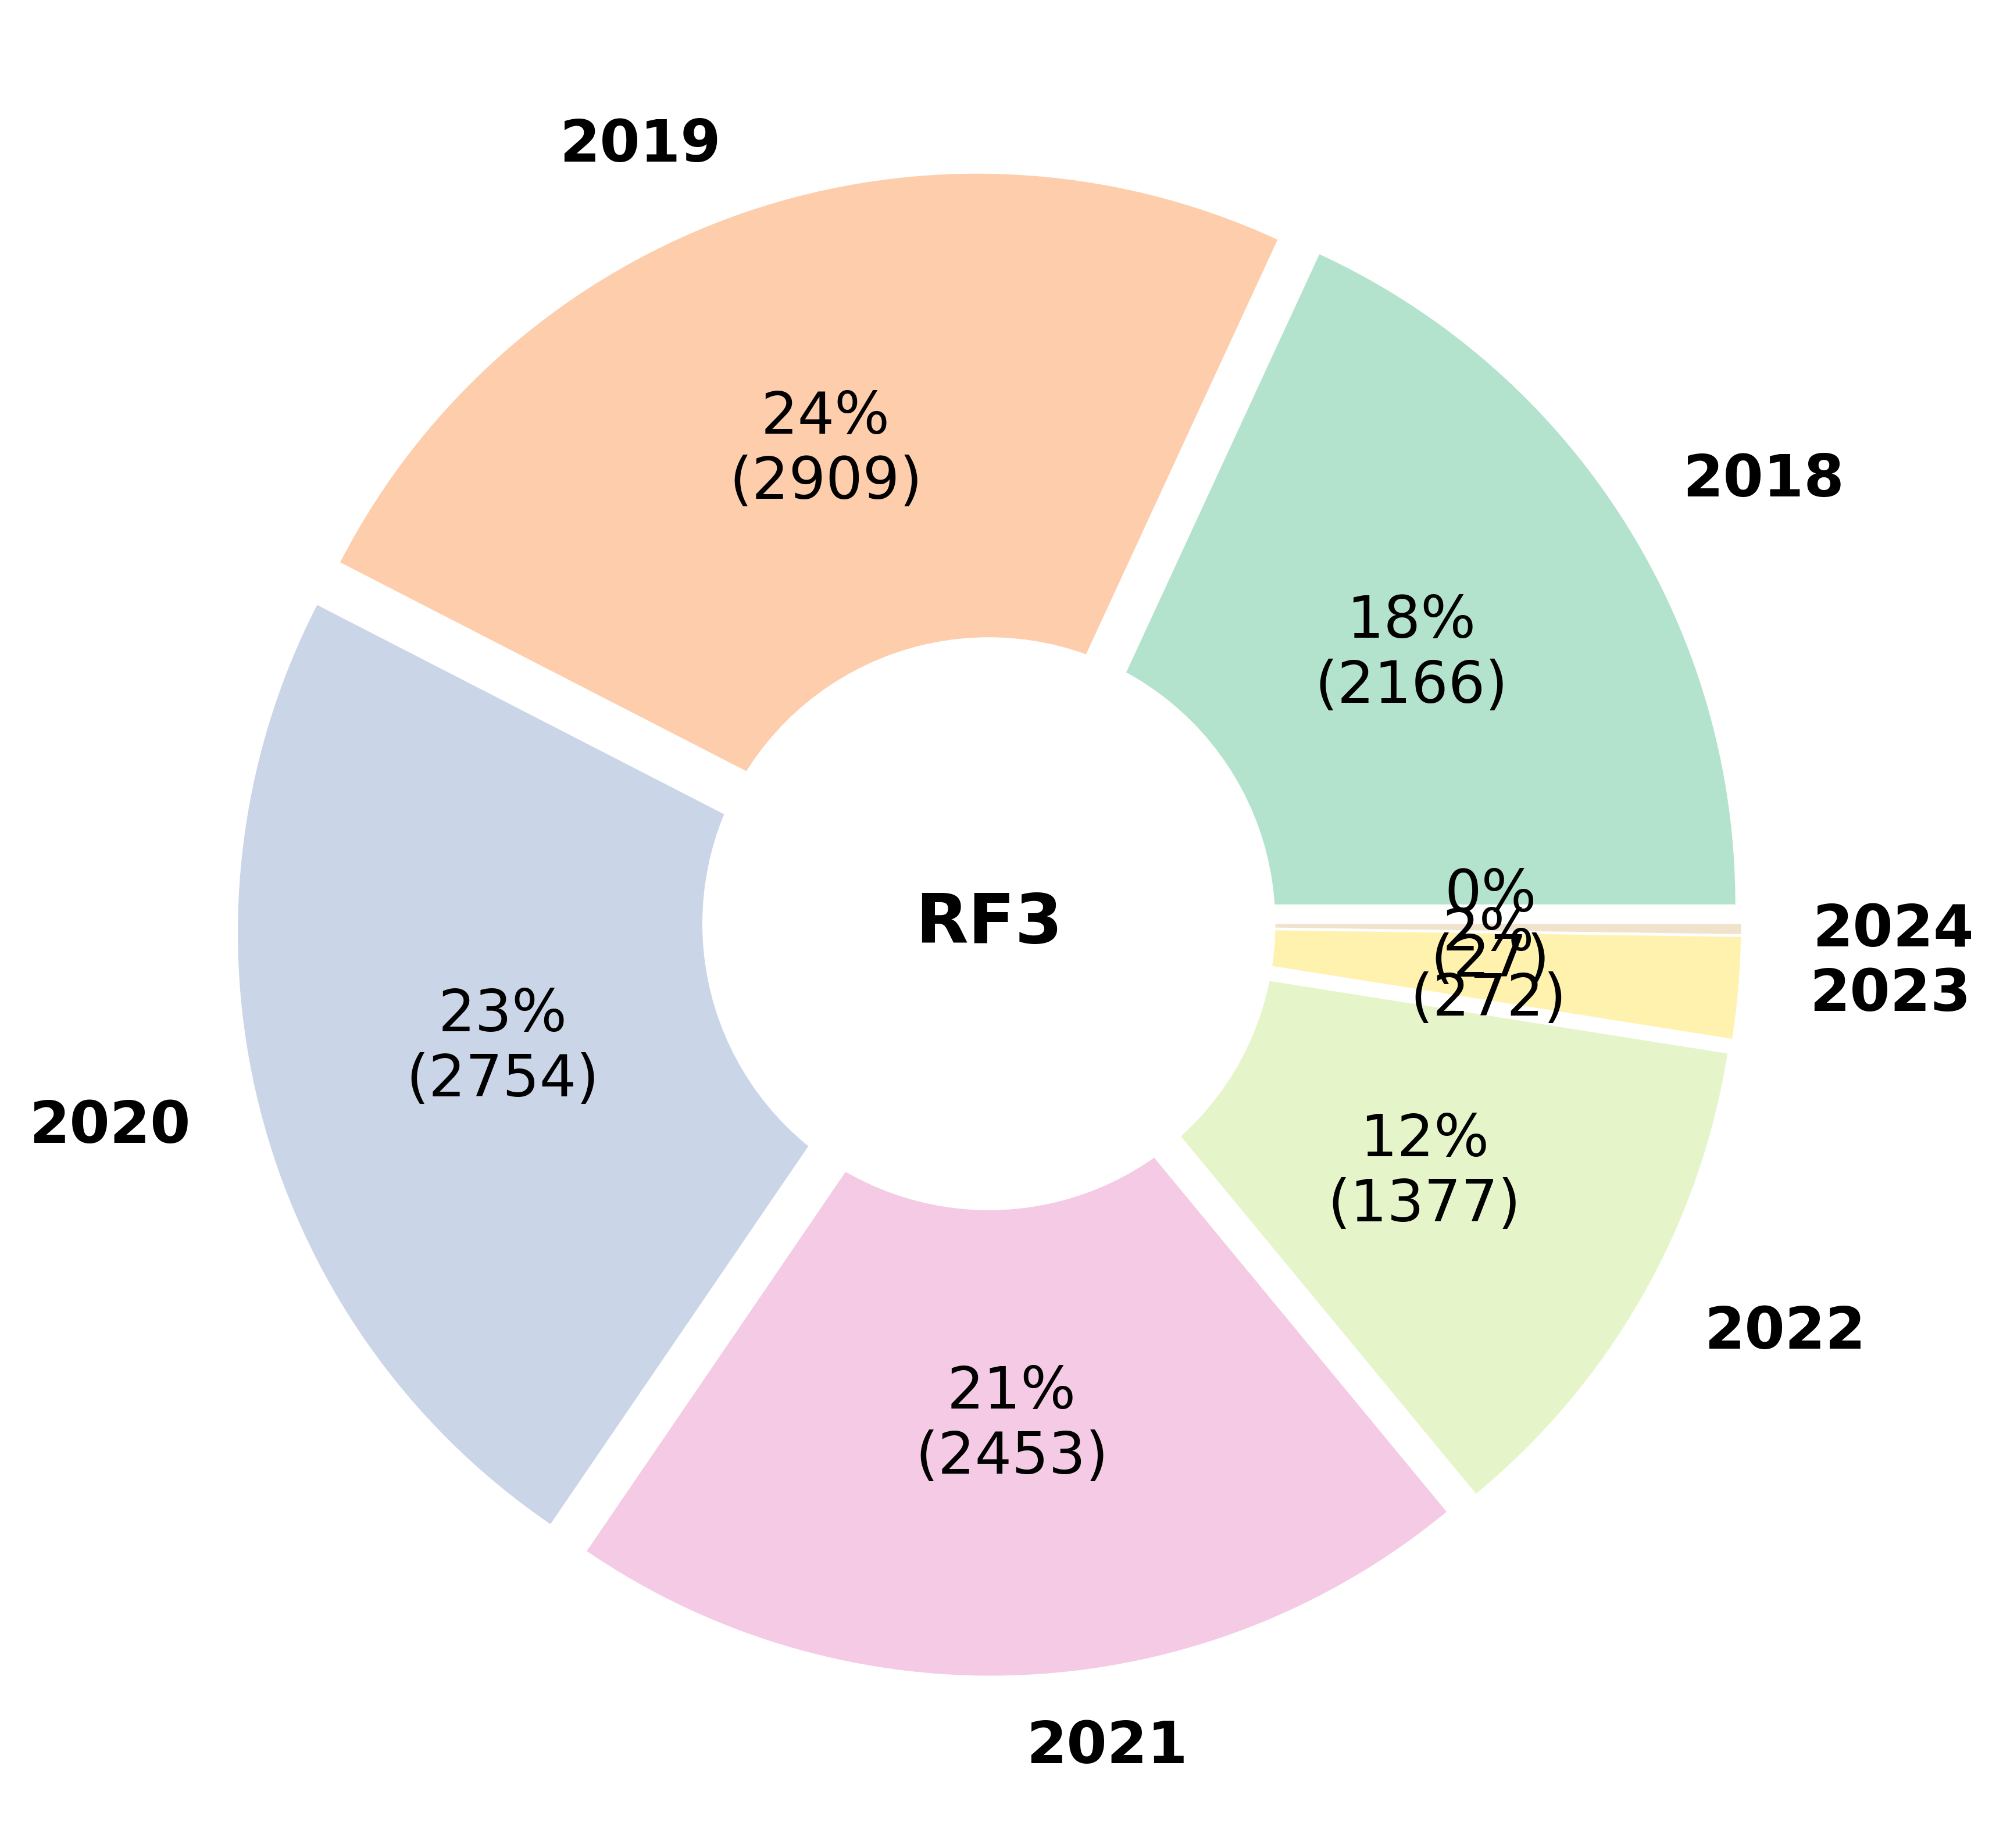
\includegraphics[width=\linewidth]{imagens/final/circle_RF3.png}
		\caption{Número de contratos inconformes detetados para o indicador RF3, por ano.}
		\label{final6}
		
	\end{minipage}
	\hfill
	\begin{minipage}{.48\linewidth}
		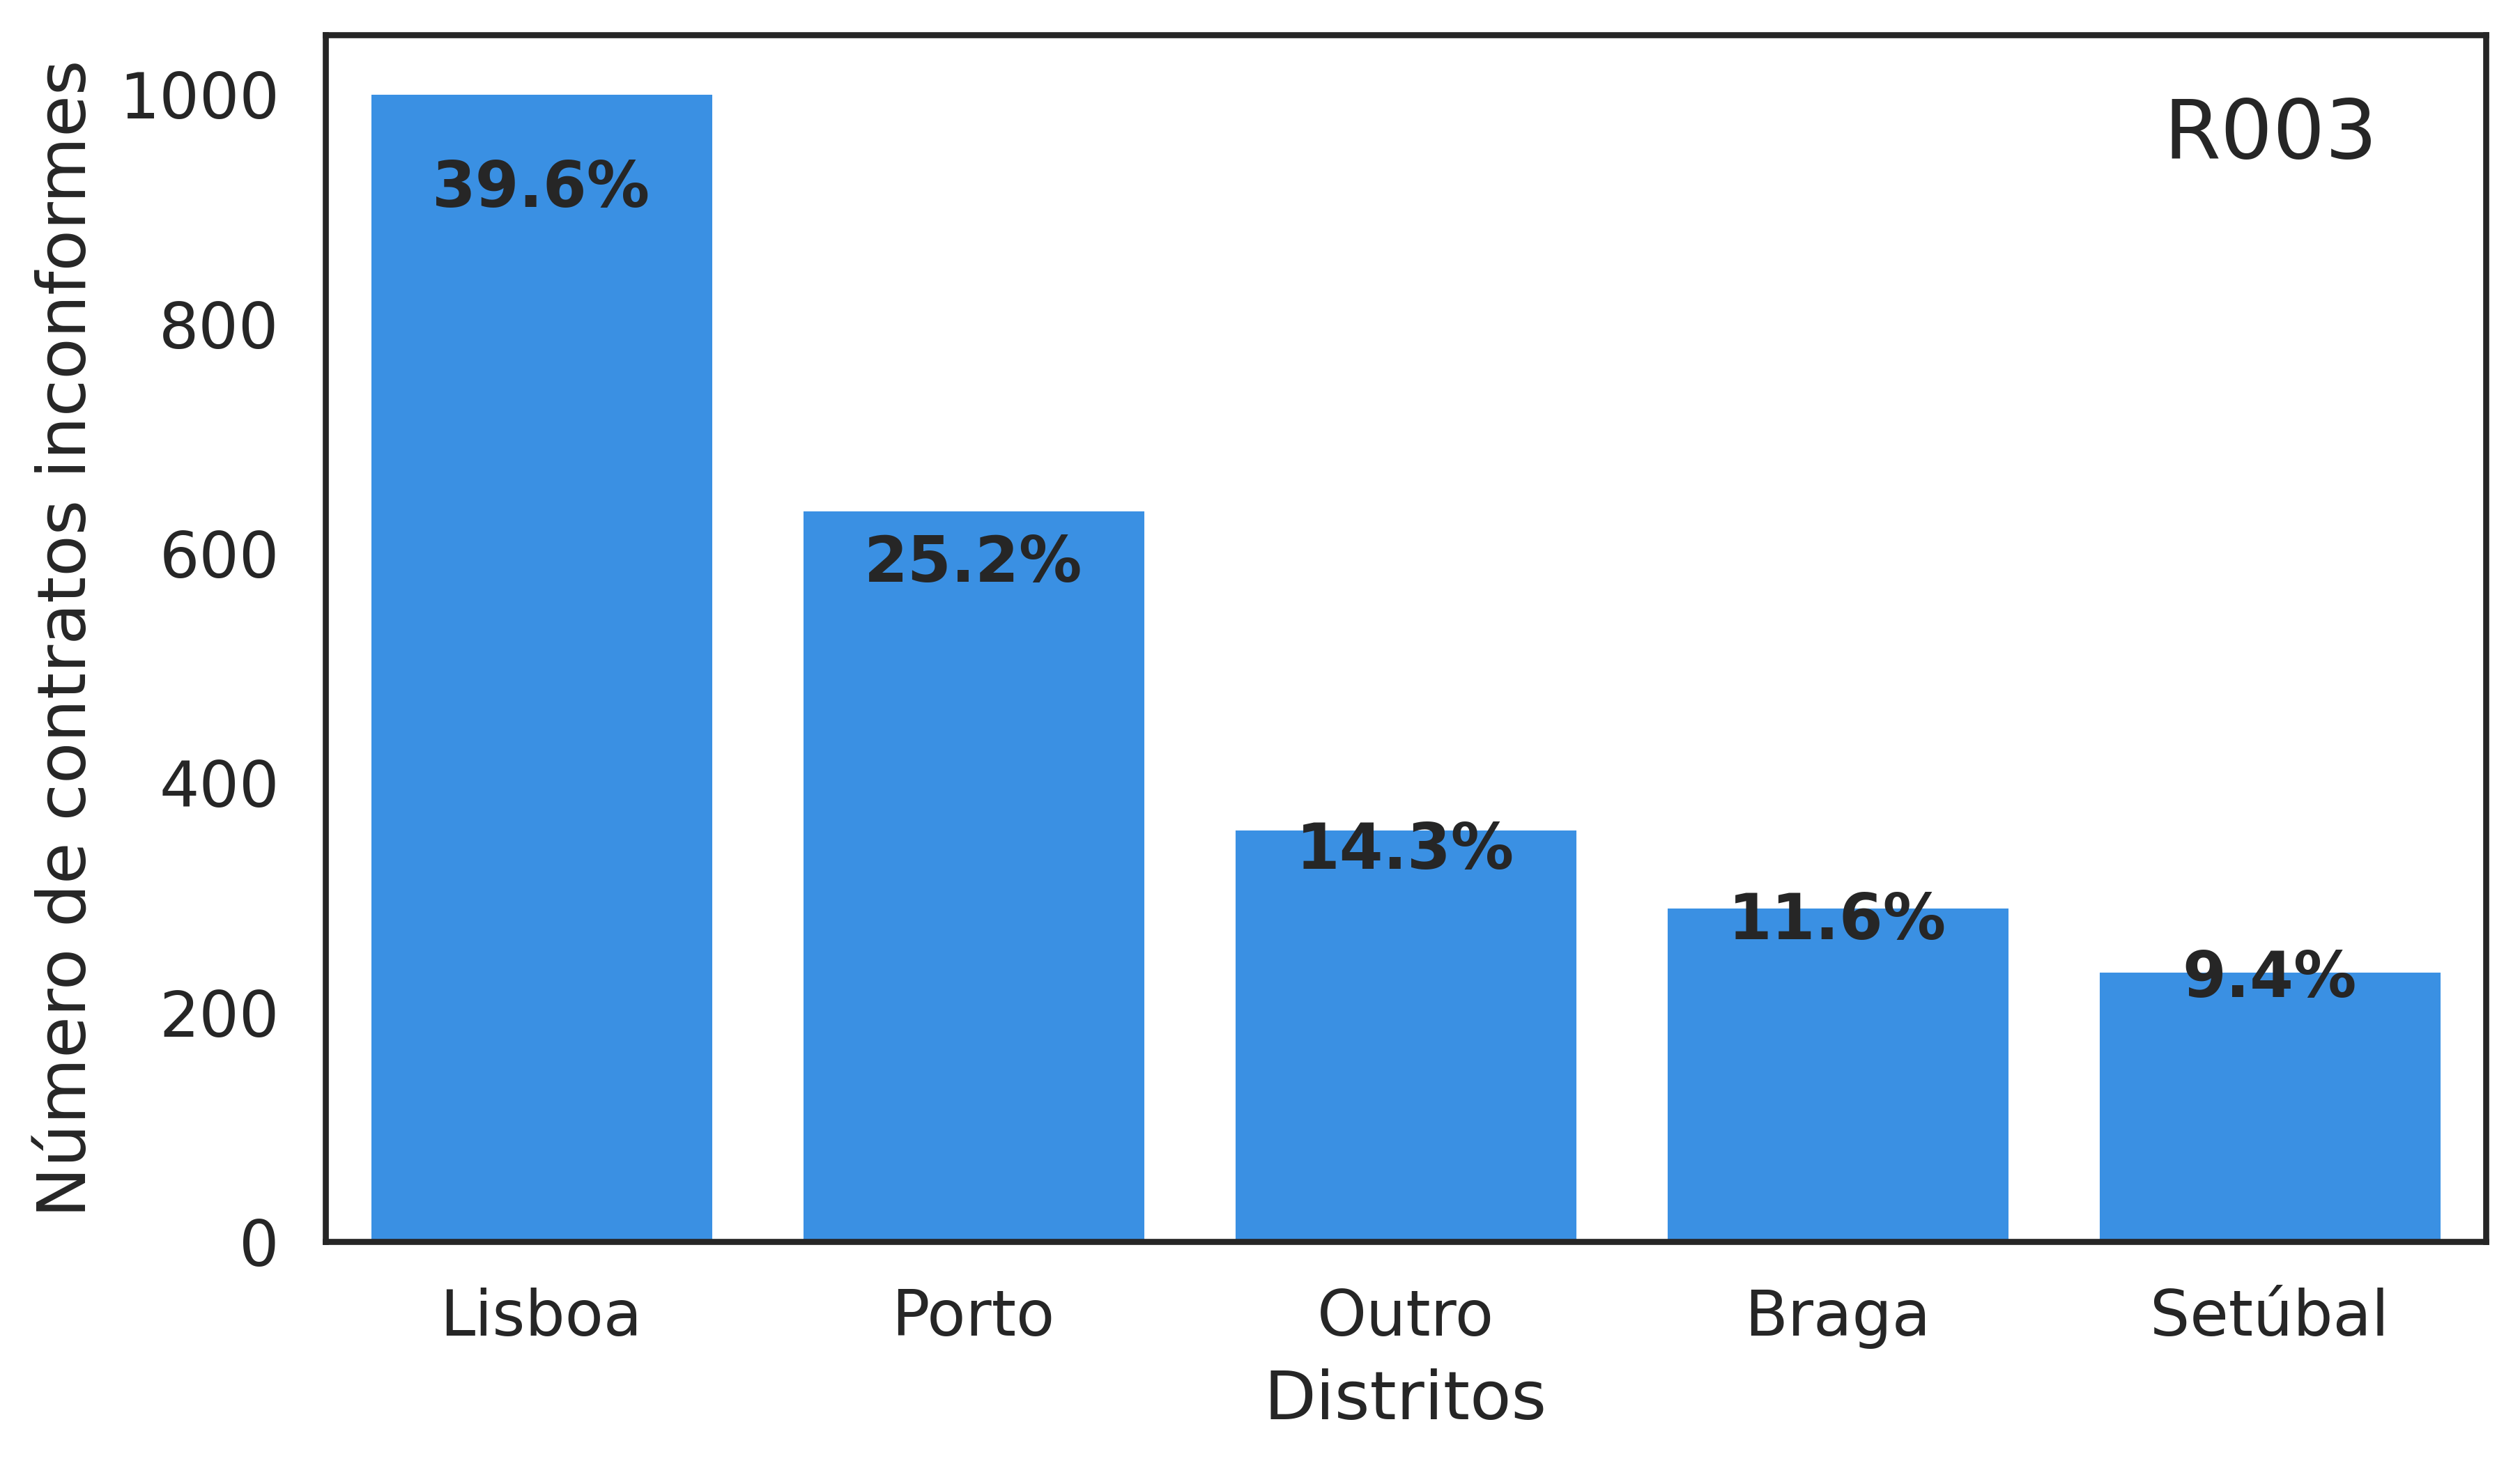
\includegraphics[width=\linewidth]{imagens/final/bar_R003.png}
		\caption{Número de contratos inconformes detetados para o indicador R003, por distrito.}
		\label{final7}
		
	\end{minipage}
\end{figure}


Nas Figuras \ref{final7}, \ref{final8}, \ref{final9}, \ref{final10} e \ref{final11} percebe-se como é que o número absoluto de contratos inconformes detetados se distribui, para cada \textit{flag}, por distrito. Concordante com a Figura INSERIR, o distrito com maior percentagem de contratos inconformes, transversal a todas as \textit{flags}, é Lisboa. Existe uma percentagem significativa de distritos caracterizados como \textit{Outro}, o que, de certa forma, deturpa os valores percentuais apresentados. Se preenchidos corretamente, verificar-se-ia um número de contratos ainda maior, possivelmente, para os distritos apresentados. Na zona norte destacam-se os distritos do Porto e Braga, enquanto que na zona sul o foco é nos distritos de Setúbal e Faro. 

\clearpage

\begin{figure}[H]
	\centering
	\begin{minipage}{.44\linewidth}
		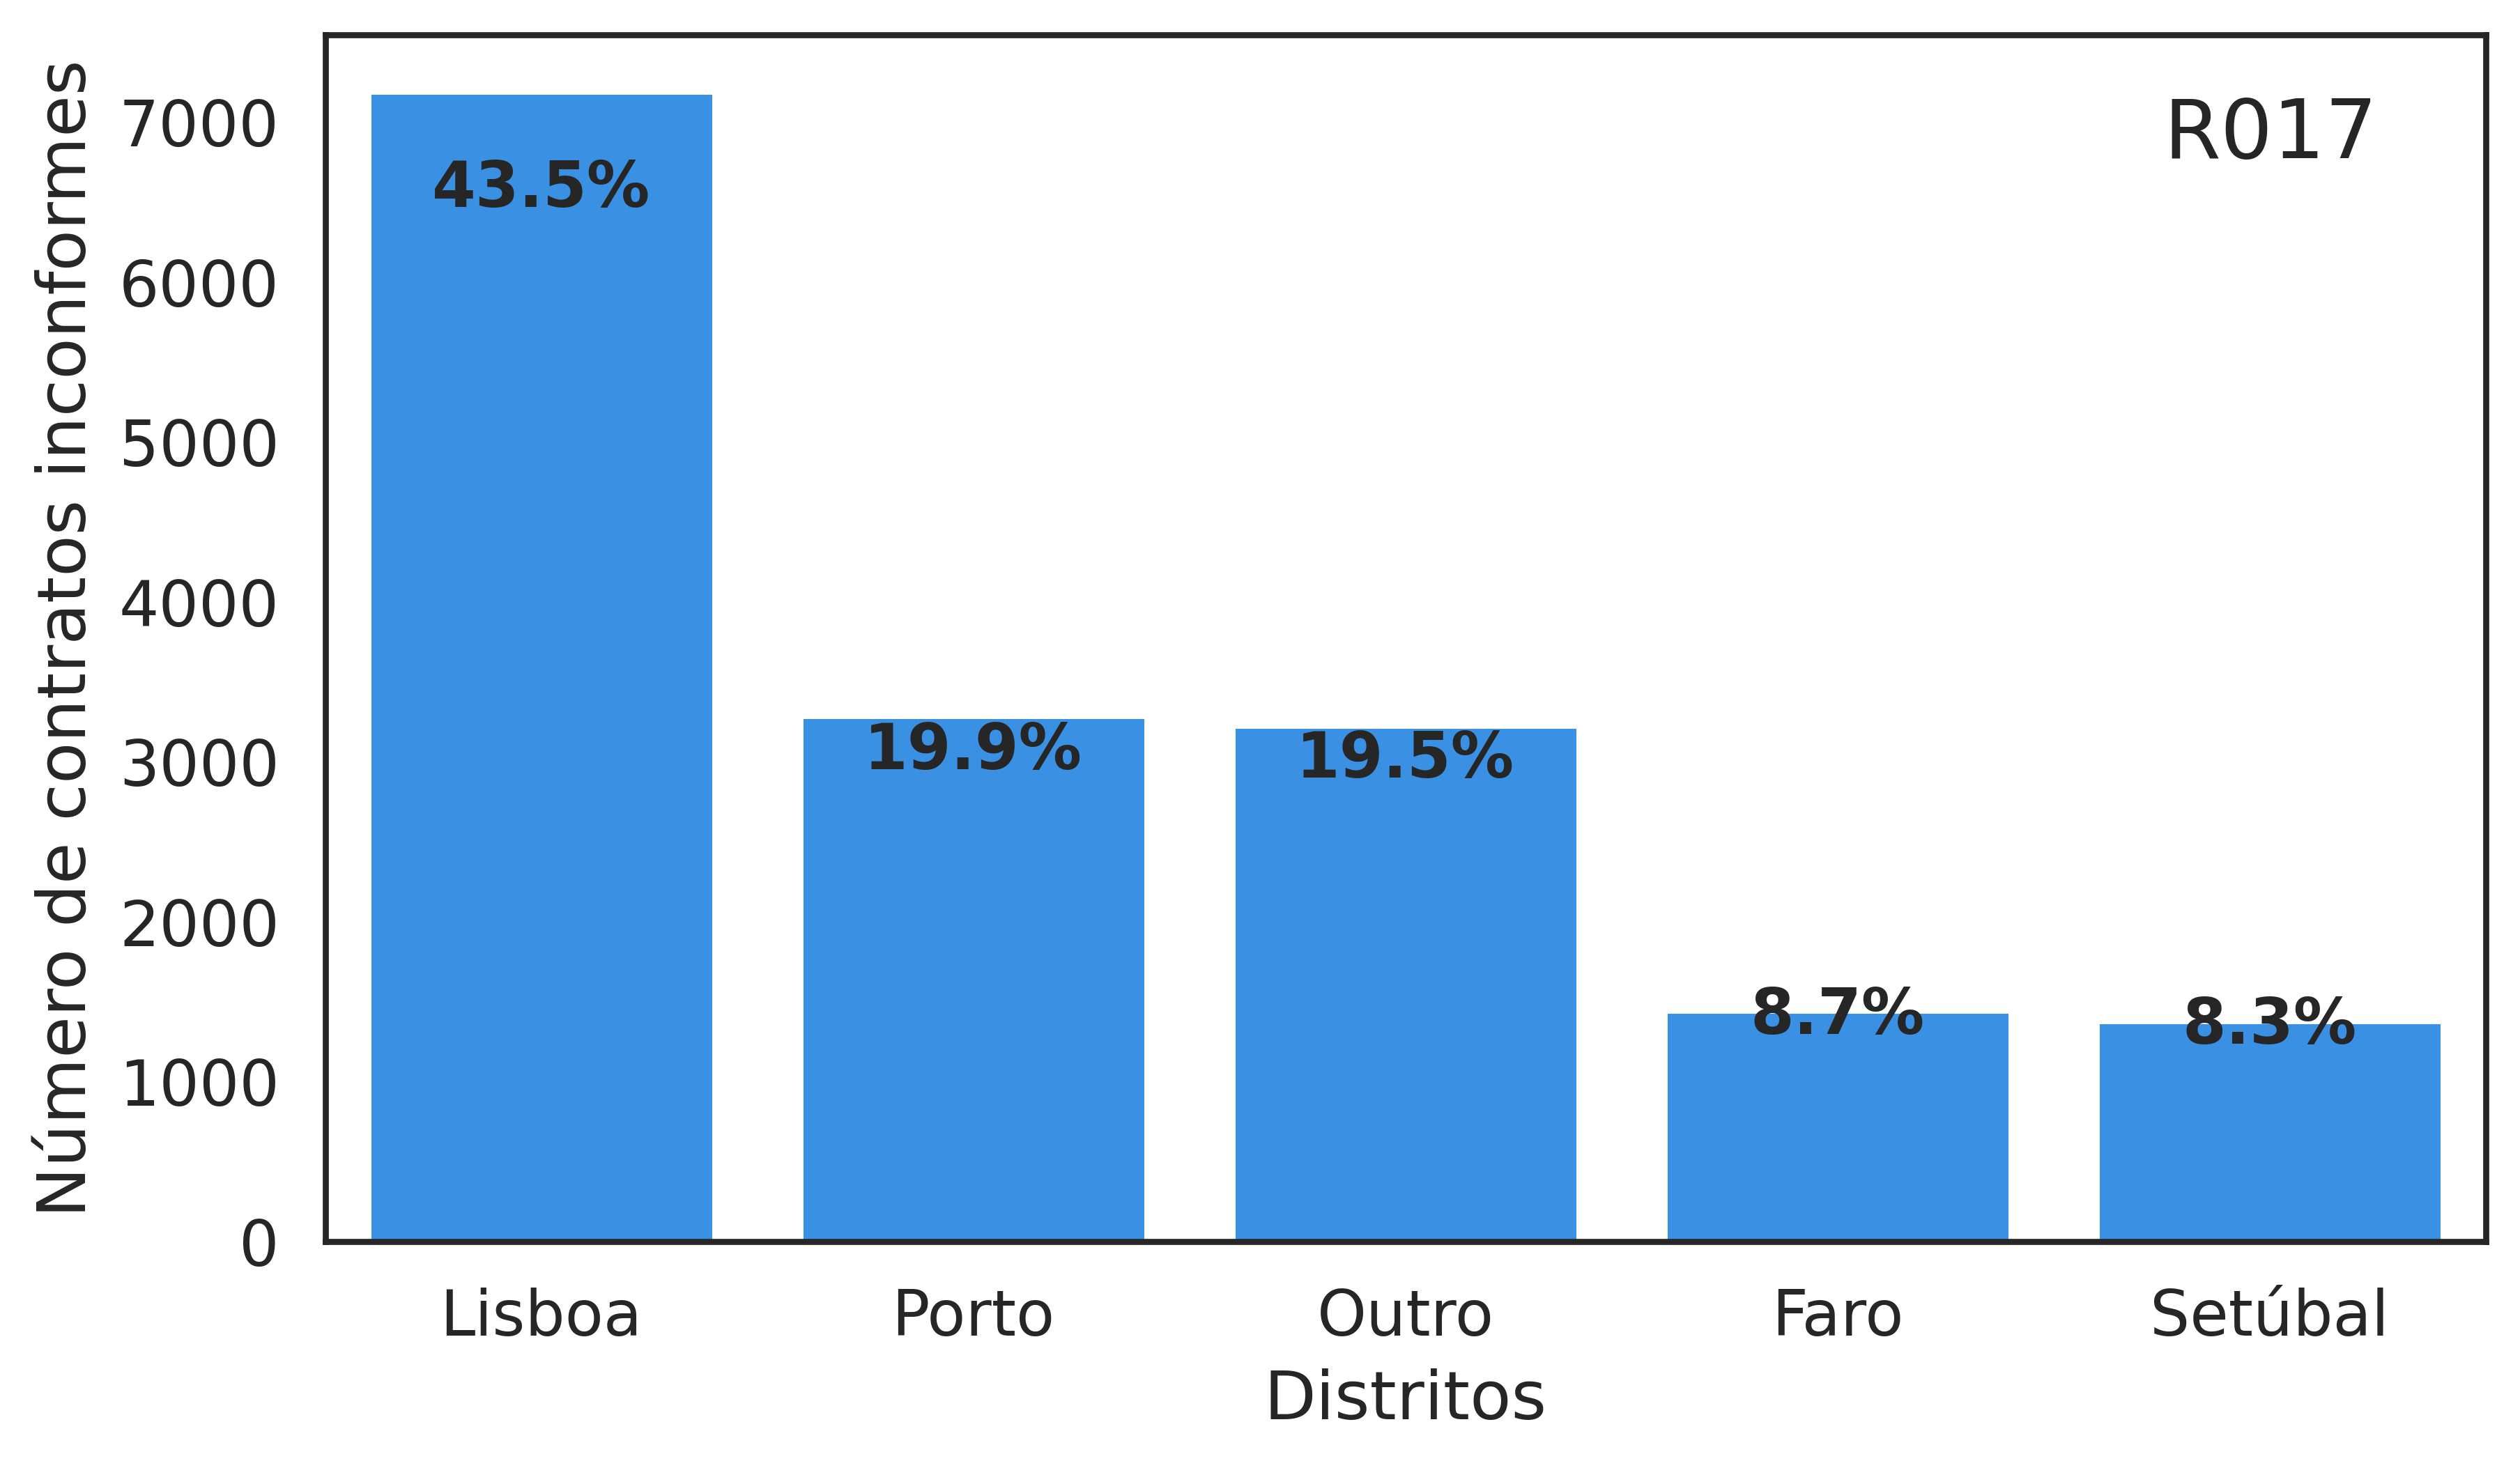
\includegraphics[width=\linewidth]{imagens/final/bar_R017.png}
				\caption{Número de contratos inconformes detetados para o indicador R017, por distrito.}
		\label{final8}
		
	\end{minipage}
	\hfill
	\begin{minipage}{.44\linewidth}
		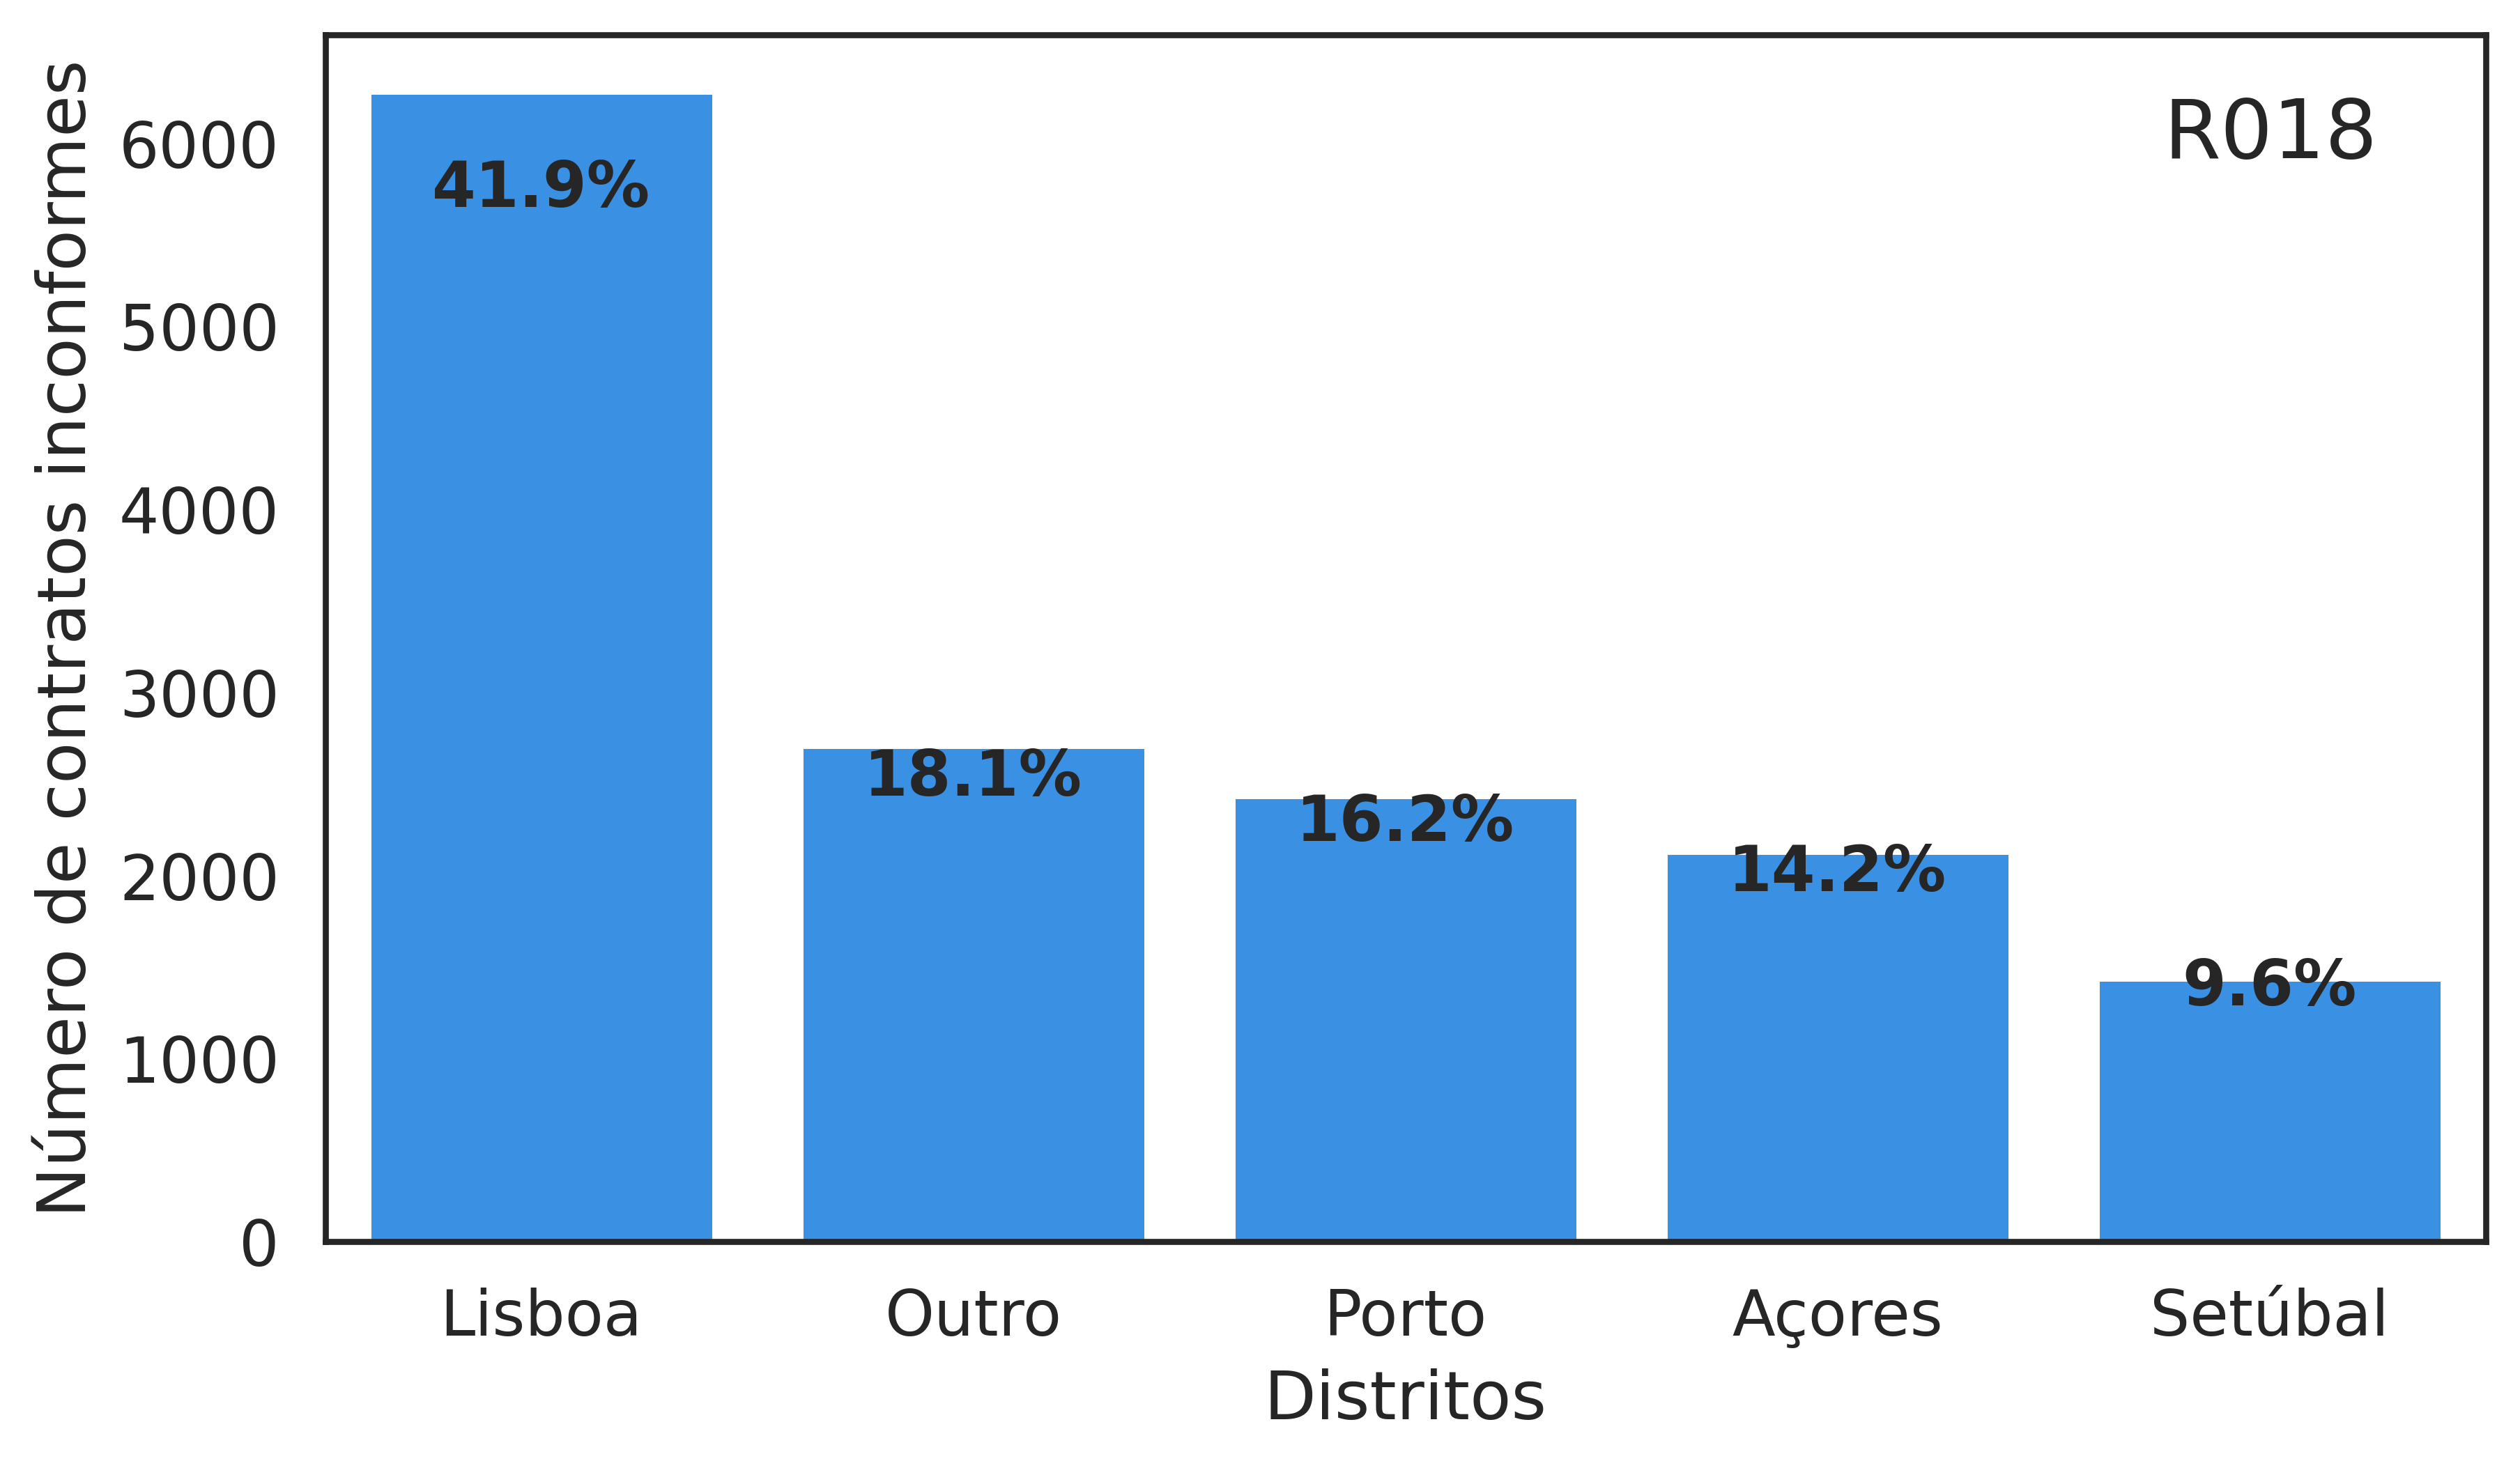
\includegraphics[width=\linewidth]{imagens/final/bar_R018.png}
		\caption{Número de contratos inconformes detetados para o indicador R018, por distrito.}
		\label{final9}
		
	\end{minipage}
\end{figure}


\begin{figure}[H]
	\centering
	\begin{minipage}{.44\linewidth}
		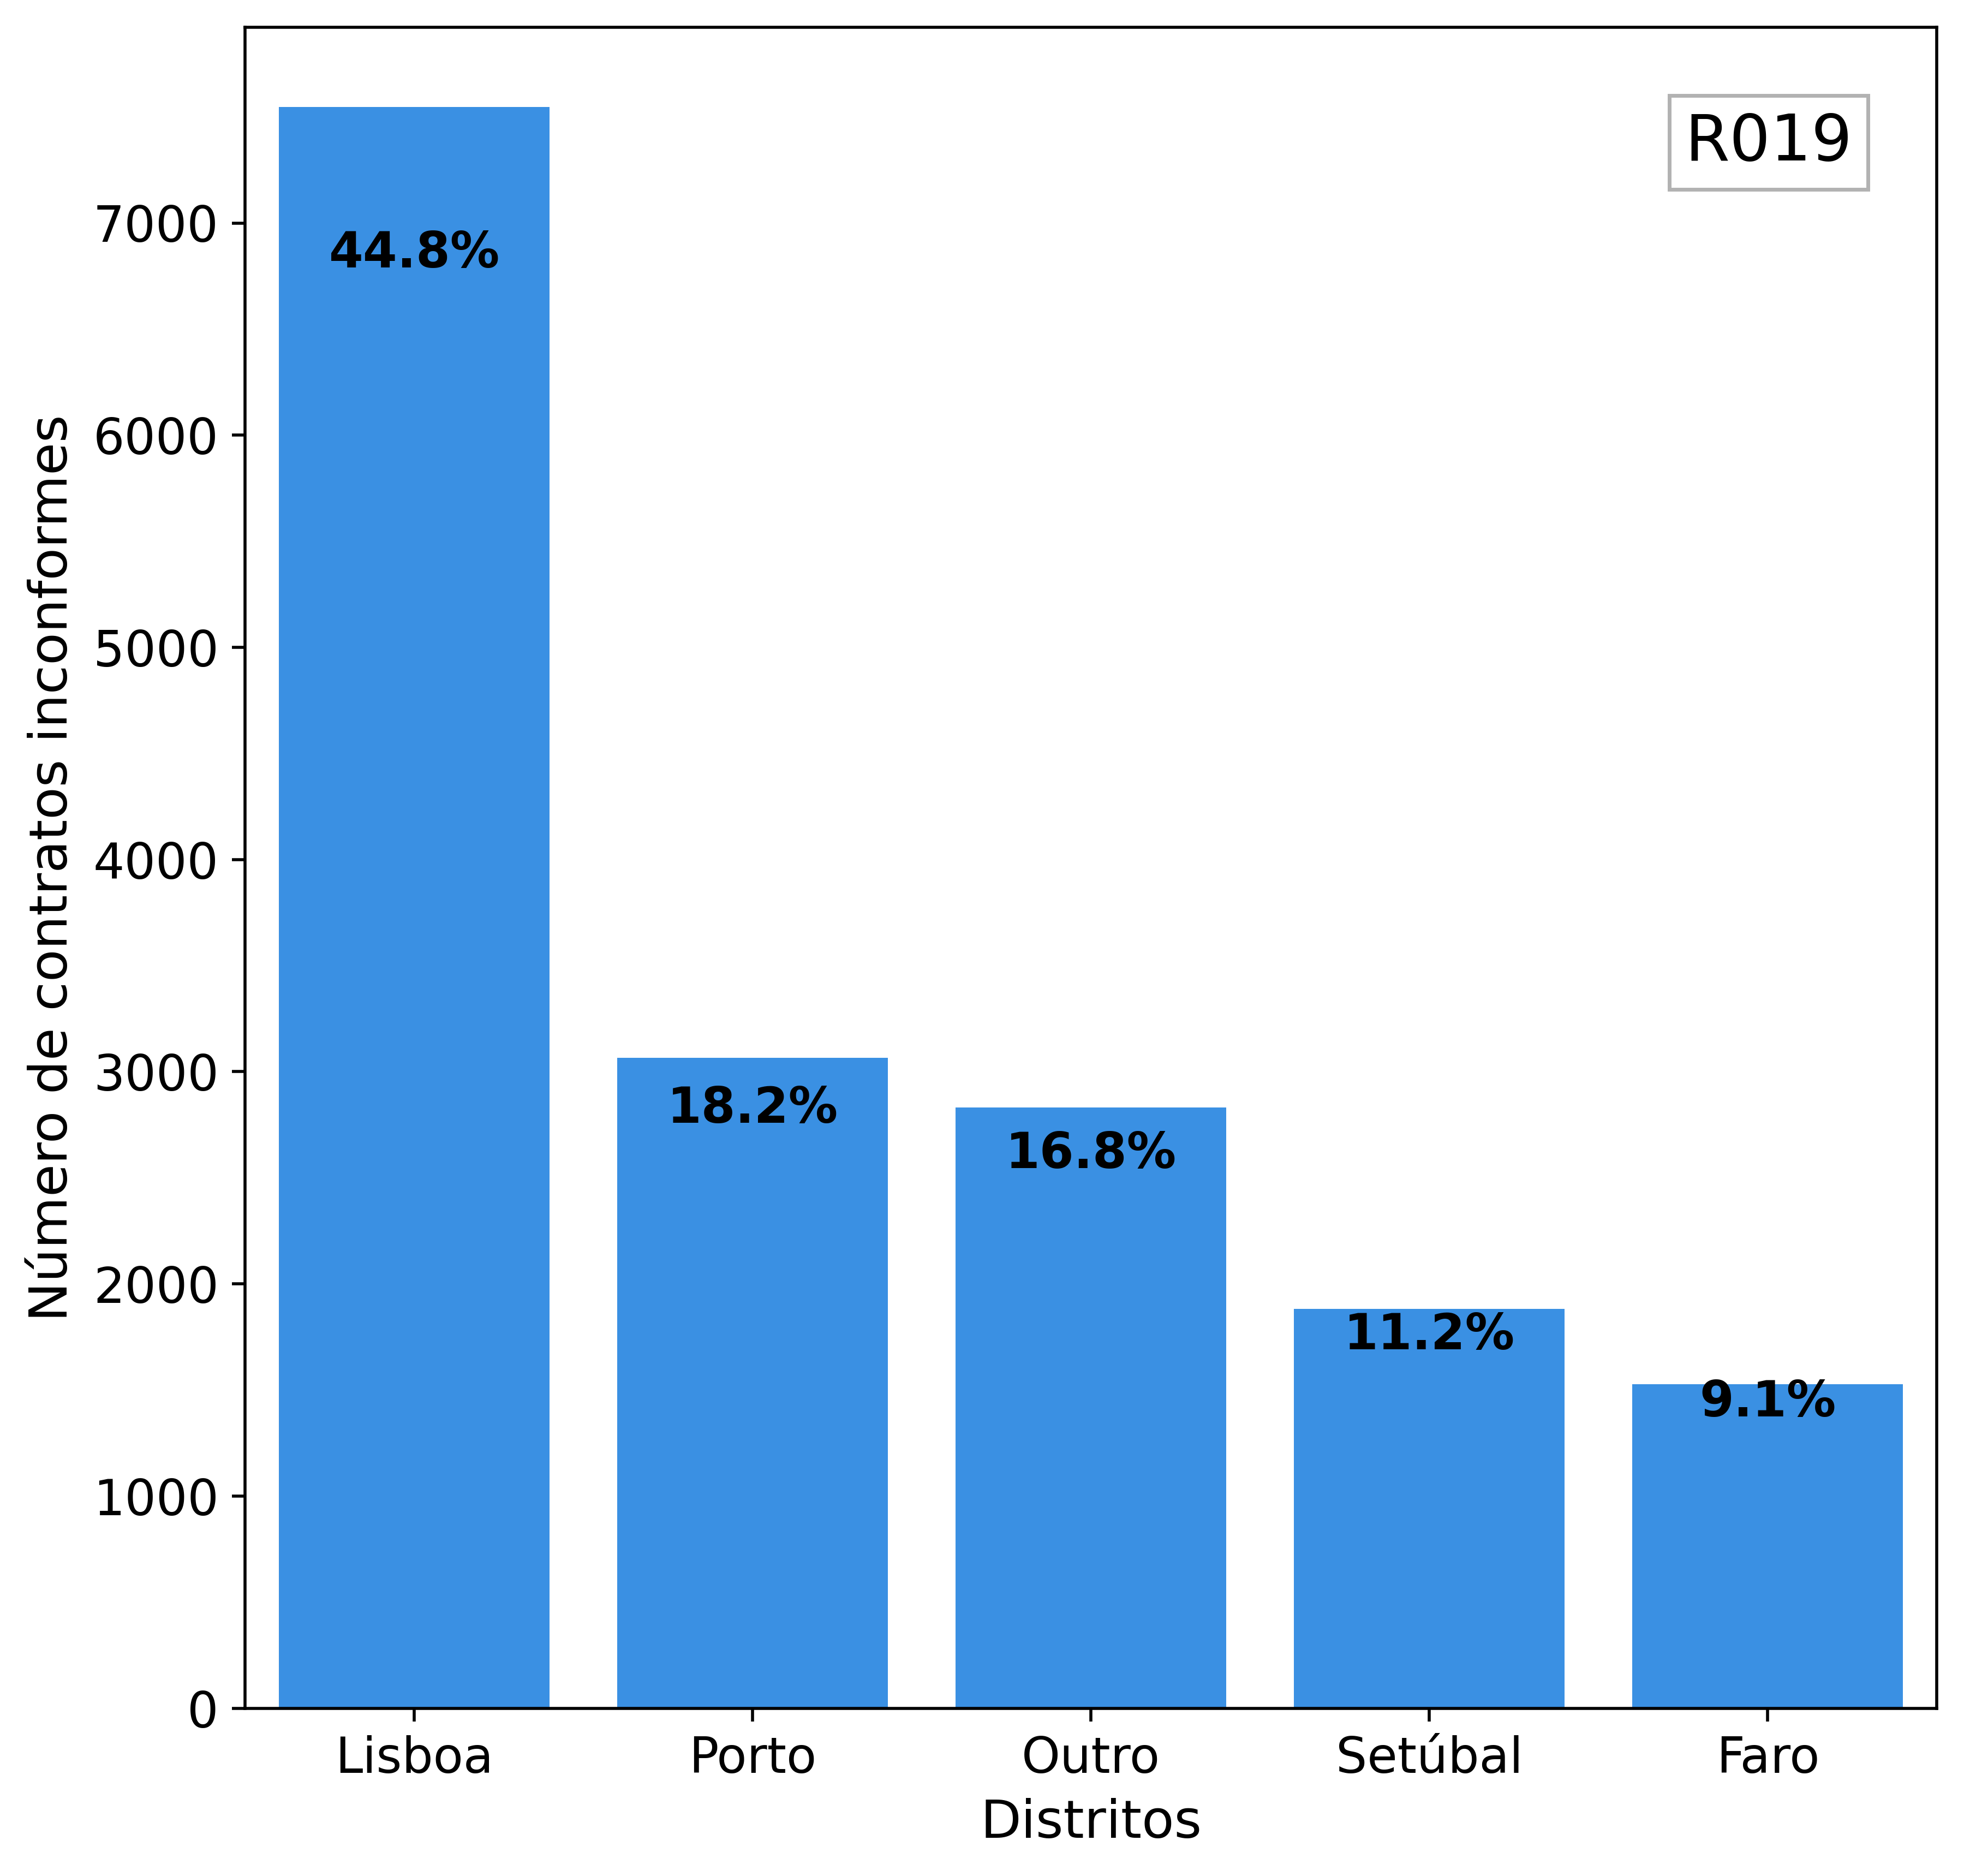
\includegraphics[width=\linewidth]{imagens/final/bar_R019.png}
		\caption{Número de contratos inconformes detetados para o indicador R019, por distrito.}
		\label{final10}
		
	\end{minipage}
	\hfill
	\begin{minipage}{.44\linewidth}
		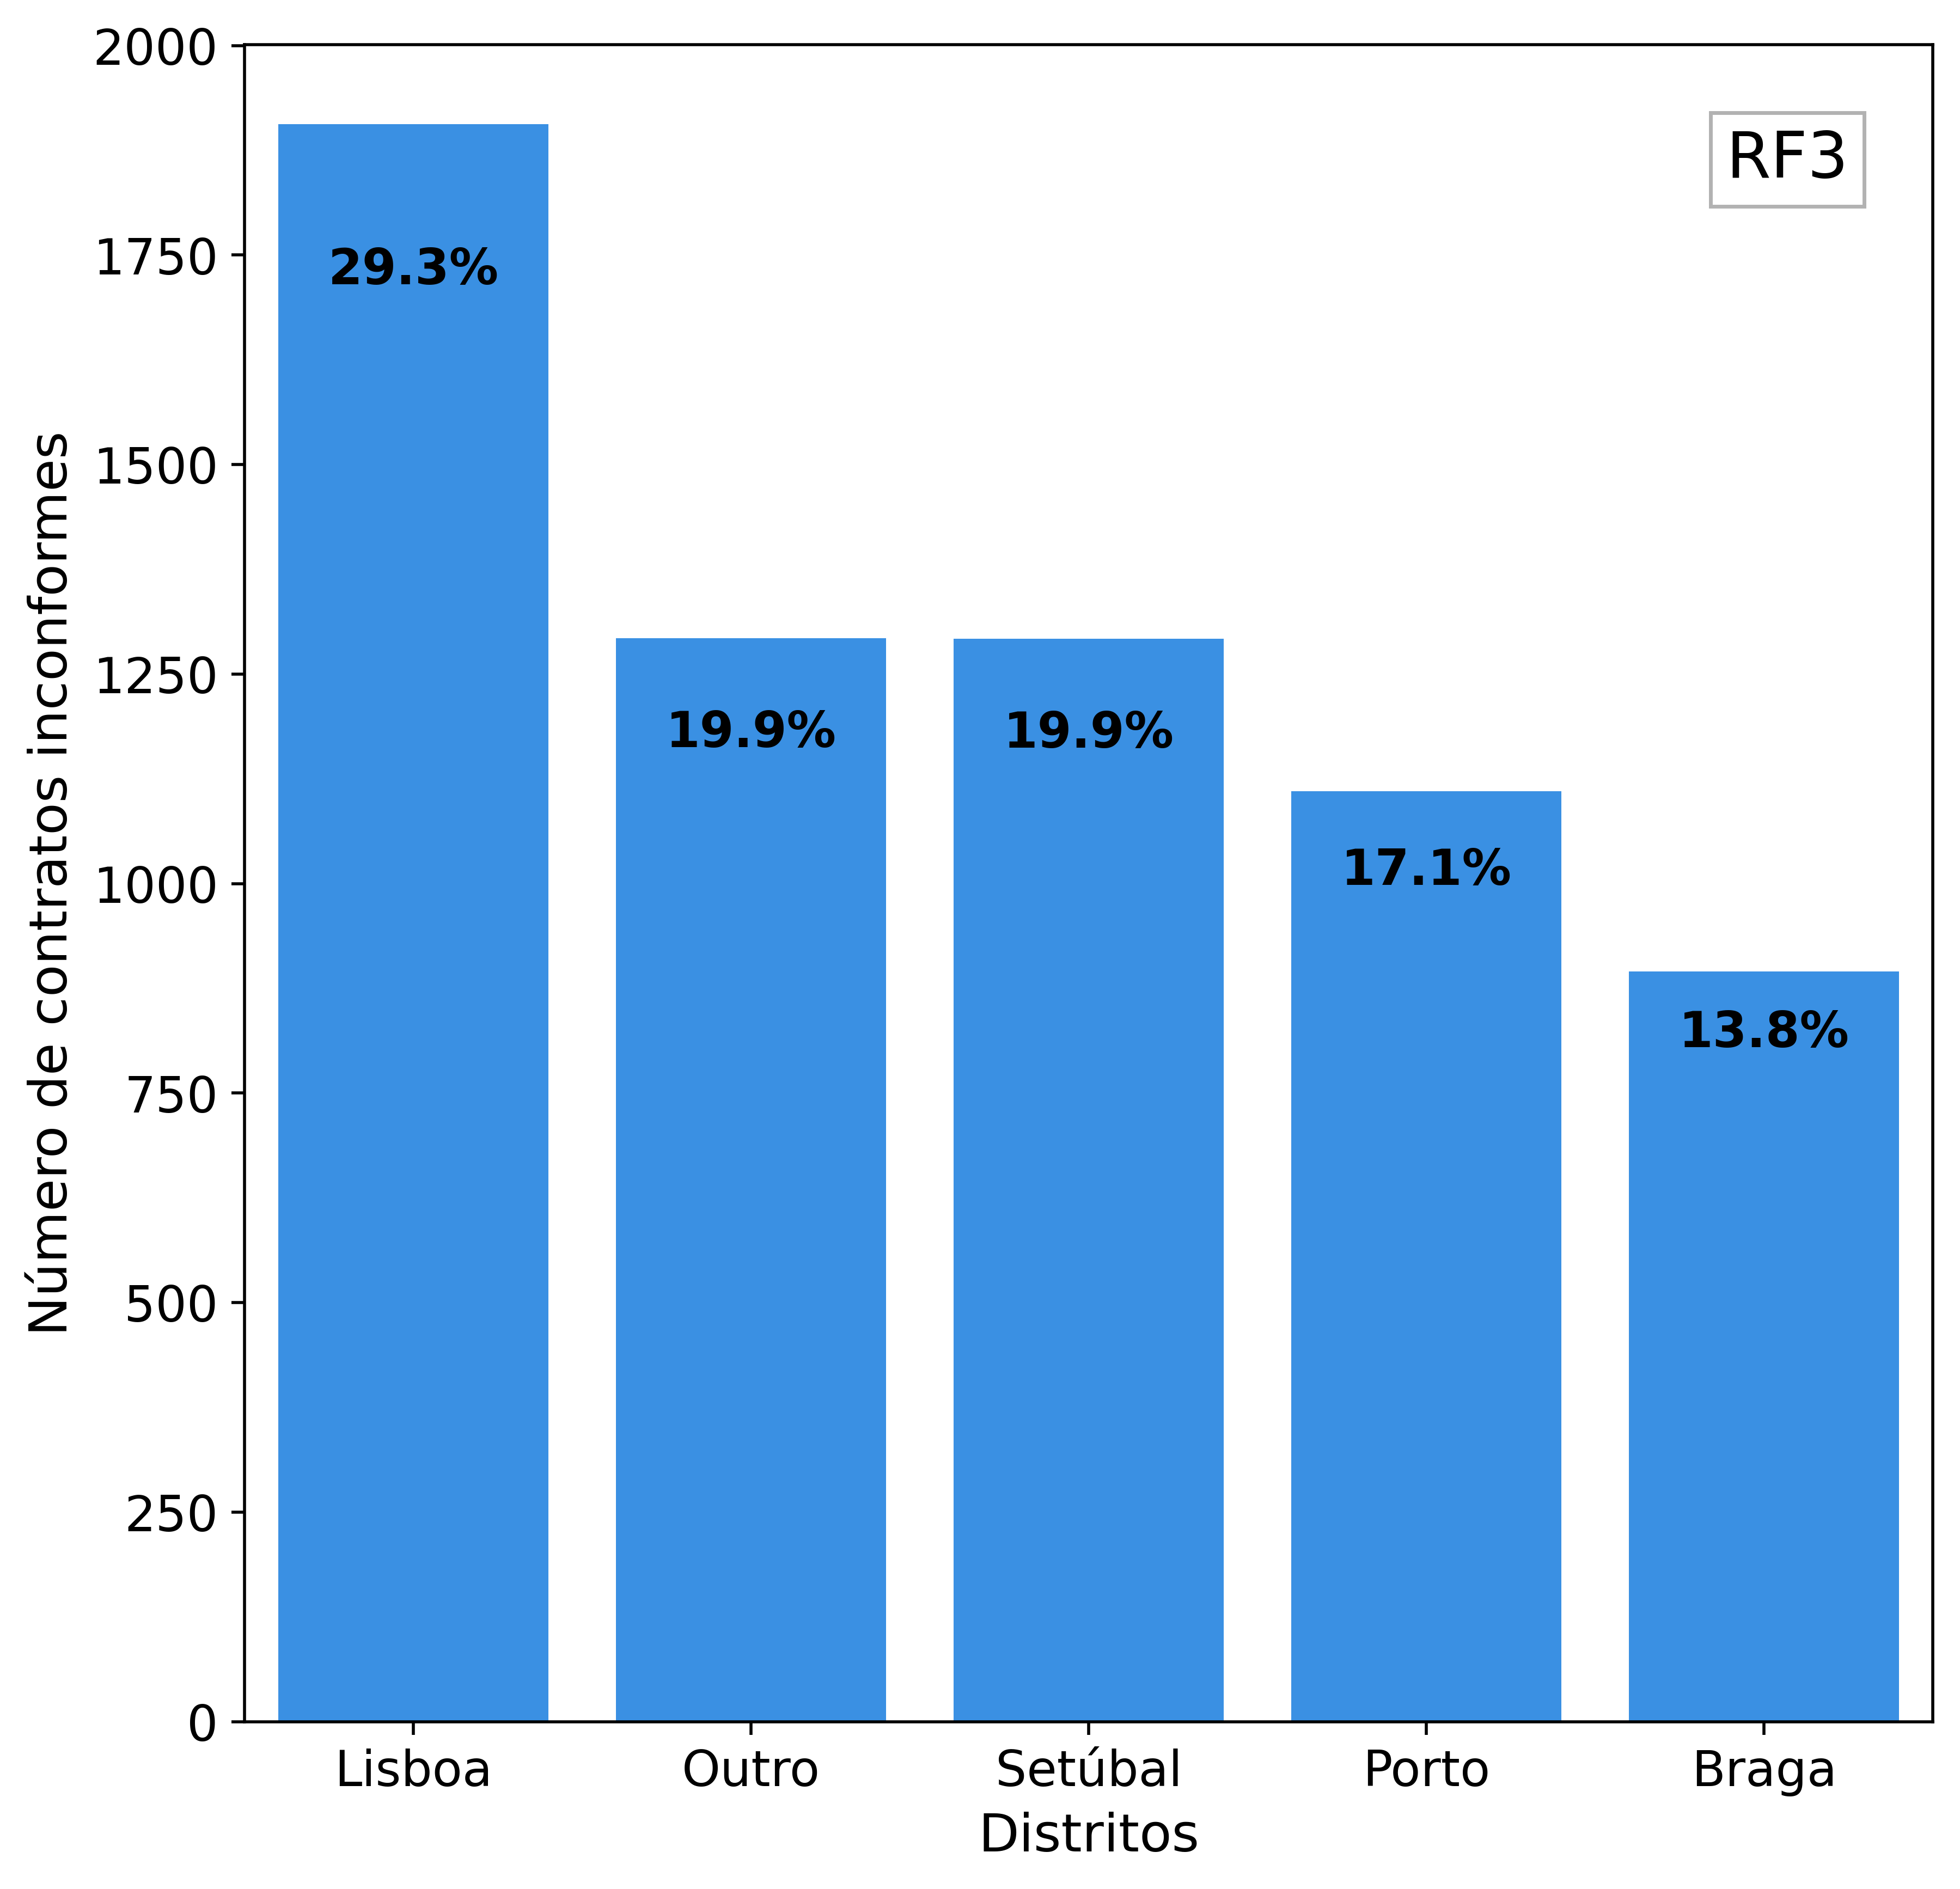
\includegraphics[width=\linewidth]{imagens/final/bar_RF3.png}
		\caption{Número de contratos inconformes detetados para o indicador RF3, por distrito.}
		\label{final11}
		
	\end{minipage}
\end{figure}


Por fim, fez-se uma contabilização do número \textit{flags} detetadas por contrato. Na Tabela \ref{final12} mostra que em 65565(50.4\%) dos contratos analisados no período de tempo considerado, não foi detetada nenhuma inconformidade. Por conseguinte, detetaram-se 39386(30.3\%) e 20589(15.8\%) contratos celebrados com uma e duas inconformidades detetadas, respetivamente. À medida que o número de inconformidades em simultâneo aumenta, o número de contraos detetados diminui. 

\begin{table}[ht]
	\centering
	\renewcommand{\arraystretch}{1.5}
	\setlength{\tabcolsep}{15pt}
	\resizebox{\textwidth}{!}{
	\begin{tabular}{cccccccc}
		\toprule
		\textbf{Número de flags}       & 0     & 1     & 2     & 3    & 4   & 5      & 6 \\ \hline
		\textbf{\begin{tabular}[c]{@{}c@{}}Número de \\ contratos detetados \end{tabular}} & 65565 & 39386 & 20589 & 5794 & 587 & 21     & 0 \\ 
		\midrule
		\textbf{Percentagem \%}                                                             & 50.4  & 30.3  & 15.8  & 4.5  & 0.5 & $<0.5$ & 0 \\ \bottomrule
	\end{tabular}%
	}
	\caption{Número de contratos, com um número variável de flags associadas, detetados.}
	\label{final12}
\end{table}














